
\documentclass[graybox,envcountchap,sectrefs]{svmono}

\usepackage{mathptmx}
\usepackage{helvet}
\usepackage{courier}
\usepackage{type1cm}
\usepackage{makeidx}   
\usepackage{graphicx}     
                            
\usepackage{multicol}     
\usepackage[bottom]{footmisc}

\usepackage{amsmath, amssymb, graphicx, graphics, float}
\usepackage{rotating}
\usepackage{sidecap}

\usepackage[colorlinks=true,citecolor=black,linkcolor=black,urlcolor=blue]{hyperref}

\newcommand{\w}{\mathbf}
\newcommand{\s}{\boldsymbol}
\newcommand{\dd}[1][n]{\left[\left[{#1}\right]\right]_{-}^{+}}

\newcommand{\delln}{\dot{\ell}^{(N)}}
\newcommand{\dell}{\dot{\ell}}
\newcommand{\elln}{\ell^{(N)}}

\newcommand{\vpv}{v_\text{\tiny{PV}}}
\newcommand{\vph}{v_\text{\tiny{PH}}}
\newcommand{\vsv}{v_\text{\tiny{SV}}}
\newcommand{\vsh}{v_\text{\tiny{SH}}}
\newcommand{\vp}{v_\text{\tiny{P}}}
\newcommand{\vs}{v_\text{\tiny{S}}}
\newcommand{\xis}{\xi_\text{\tiny{S}}}
\newcommand{\xip}{\xi_\text{\tiny{P}}}
\newcommand{\vpi}{\bar{v}_\text{\tiny{P}}}
\newcommand{\vsi}{\bar{v}_\text{\tiny{S}}}
\newcommand{\tr}{\text{tr}\,}
\newcommand{\R}{\mathbb{R}}
\newcommand{\tu}{\tilde{u}_i}
\newcommand{\sign}{\text{sign\,}}
\newcommand{\p}{\partial}

\newcommand{\bpsi}{\bar{\psi}}
\newcommand{\bphi}{\bar{\phi}}

\newcommand{\SES}{\texttt{SES3D}$\,$}

%%%%%%%%%%%%%%%%%%%%%%%%%%%%%%%%%%%%%%%%%%%%%%%%%%%%%%%%%%%%%%%%%%%%%

\begin{document}

\title{ 	\Huge{\textbf{SES3D} version 4.1}\\[10pt] 
	\large{Documentation}\\[100pt]
	\LARGE{Andreas Fichtner}\\[5pt] 
	\normalsize{Department of Earth Sciences, ETH Zurich, Switzerland}\\[15pt]
	\LARGE{Lion Krischer}\\[5pt]
	\normalsize{Department of Earth and Environmental Sciences, LMU Munich, Germany}\\[90pt]
	\normalsize{31 March 2014} }

\maketitle

\frontmatter%%%%%%%%%%%%%%%%%%%%%%%%%%%%%%%%%%%%%%%%%%%%%%%%%%%%%%%%%%%%%%%

\tableofcontents

\foreword

\SES is a programme package for the simulation of elastic wave
propagation and waveform inversion in a spherical section. The package is based on a spectral-element discretisation of
the seismic wave equation combined with adjoint techniques.\\[5pt]
\SES supports 3D heterogeneous visco-elastic rheologies with radial anisotropy. Anisotropic perfectly matched layers
are implemented to avoid reflections from the unphysical boundaries of the spherical section.\\[5pt]
\SES operates in the natural spherical coordinates, which is untypical for spectral-element approaches. The advantages are a
compact programme code, fast computations for spherical sections that are sufficiently far
from the poles and the core, and the easy implementation of 3D models.\\[5pt]
\SES is fully parallelised, meaning that the computational domain is partitioned into subdomains, each of which is assigned to one compute core. Communication between subdomains is based on MPI.\\[5pt]
\SES has been developed for continental-scale full seismic waveform
inversion. It is, however, applicable to a wide range of local- to continental-scale wave propagation problems.\\[5pt]
\SES is deliberately puristic. This is intended to (1) make the code
easily adaptable to particular problems, (2) facilitate the
implementation of 3D models, (3) reduce the likelihood of
programming errors, and (4) allow for an easy adaptation to new hardware architectures. The last point becomes particularly relevant in times when hardware architecture changes rapidly.\\[5pt]
This tutorial is split into a description of the programme code and
an introduction to the mathematical background of \SES. Reading the
mathematical part is not required to successfully run \SES. It is,
however, strongly recommended. The chance of using \SES incorrectly
or inefficiently is high when its mathematical background is not
known. This is true for any numerical method.\\[5pt]
The description of the programme package is centred around
realistic examples that a new user may want to reproduce in order to
become familiar with \SES.\\[5pt]
\textbf{\SES is hosted on} \href{https://github.com}{Github} \textbf{and can be obtained from} \href{https://github.com/echolite/ses3d}{https://github.com/echolite/ses3d}.


\vspace{\baselineskip}
\begin{flushright}\noindent
Zurich, February 2014\hfill {\it Andreas Fichtner}\\
\end{flushright}


\mainmatter%%%%%%%%%%%%%%%%%%%%%%%%%%%%%%%%%%%%%%%%%%%%%%%%%%%%%%%%%%%%%%%

%- code description %%%%%%%%%%%%%%%%%%%%%%%%%%%%%%%%%%%%%%%%%%%%%%%%%%%%%%%%%%%

\begin{partbacktext}
\part{Code description}


\end{partbacktext}
      
	
	\chapter{Code structure}

%====================================================================
% Directory structure.
%====================================================================

\section{Directory structure}

Figure \ref{F:directory_structure} illustrates the directory structure of \SES. The contents of the different directories are as
follows:\\[5pt]
\texttt{ADJOINT:} Adjoint source time functions and a list of adjoint source locations.\\[5pt]
\texttt{DATA/COORDINATES:} ASCII files containing the grid point coordinates for each model subdomain.\\[5pt]
\texttt{DATA/LOGFILES:} Logfiles for each model subdomain. Logfiles document the geometrical setup of each subdomain and the iteration progress. They are mostly used for debugging.\\[5pt]
\texttt{DATA/OUTPUT:} Directory reserved for output such as seismograms, 3D wavefield snapshots and 3D sensitivity kernels.\\[5pt]
\texttt{INPUT:} Input files: \texttt{setup} (model geometry and parallelisation), \texttt{event\_1, event\_2, ...} (event files, one for each earthquake to be modelled, source parameters, output directory, time stepping variables), \texttt{event\_list} (list of events to be modelled), \texttt{recfile} (list of receiver locations), \texttt{stf} (source time function)\\[5pt]
\texttt{MAIN:} Executables for \SES wave propagation.\\[5pt]
\texttt{SOURCE:} Fortran source files for \SES wave propagation.\\[5pt]
\texttt{MODELS/MAIN:} Executables for the generation of Earth models.\\[5pt]
\texttt{MODELS/MODELS:} Physical model parameters. One file for each compute core. Read by the wave propagation executables.\\[5pt]
\texttt{MODELS/MODELS\_1D:} Fortran codes for the implementation of a selection of 1D Earth models.\\[5pt]
\texttt{MODELS/MODELS\_3D:} 3D Earth models or Earth model perturbations.\\[5pt]
\texttt{MODELS/SOURCE:} Source code for Earth model generation. \\[5pt]
\texttt{TOOLS:} Collection of Fortran and Python tools for visualisation, model manipulation and the computation of adjoint sources.\\[5pt]
\texttt{SCENARIOS:} Input files for the \SES scenarios described in this tutorial.
%========================================================================
\begin{center}
\begin{figure}
\center\scalebox{0.15}{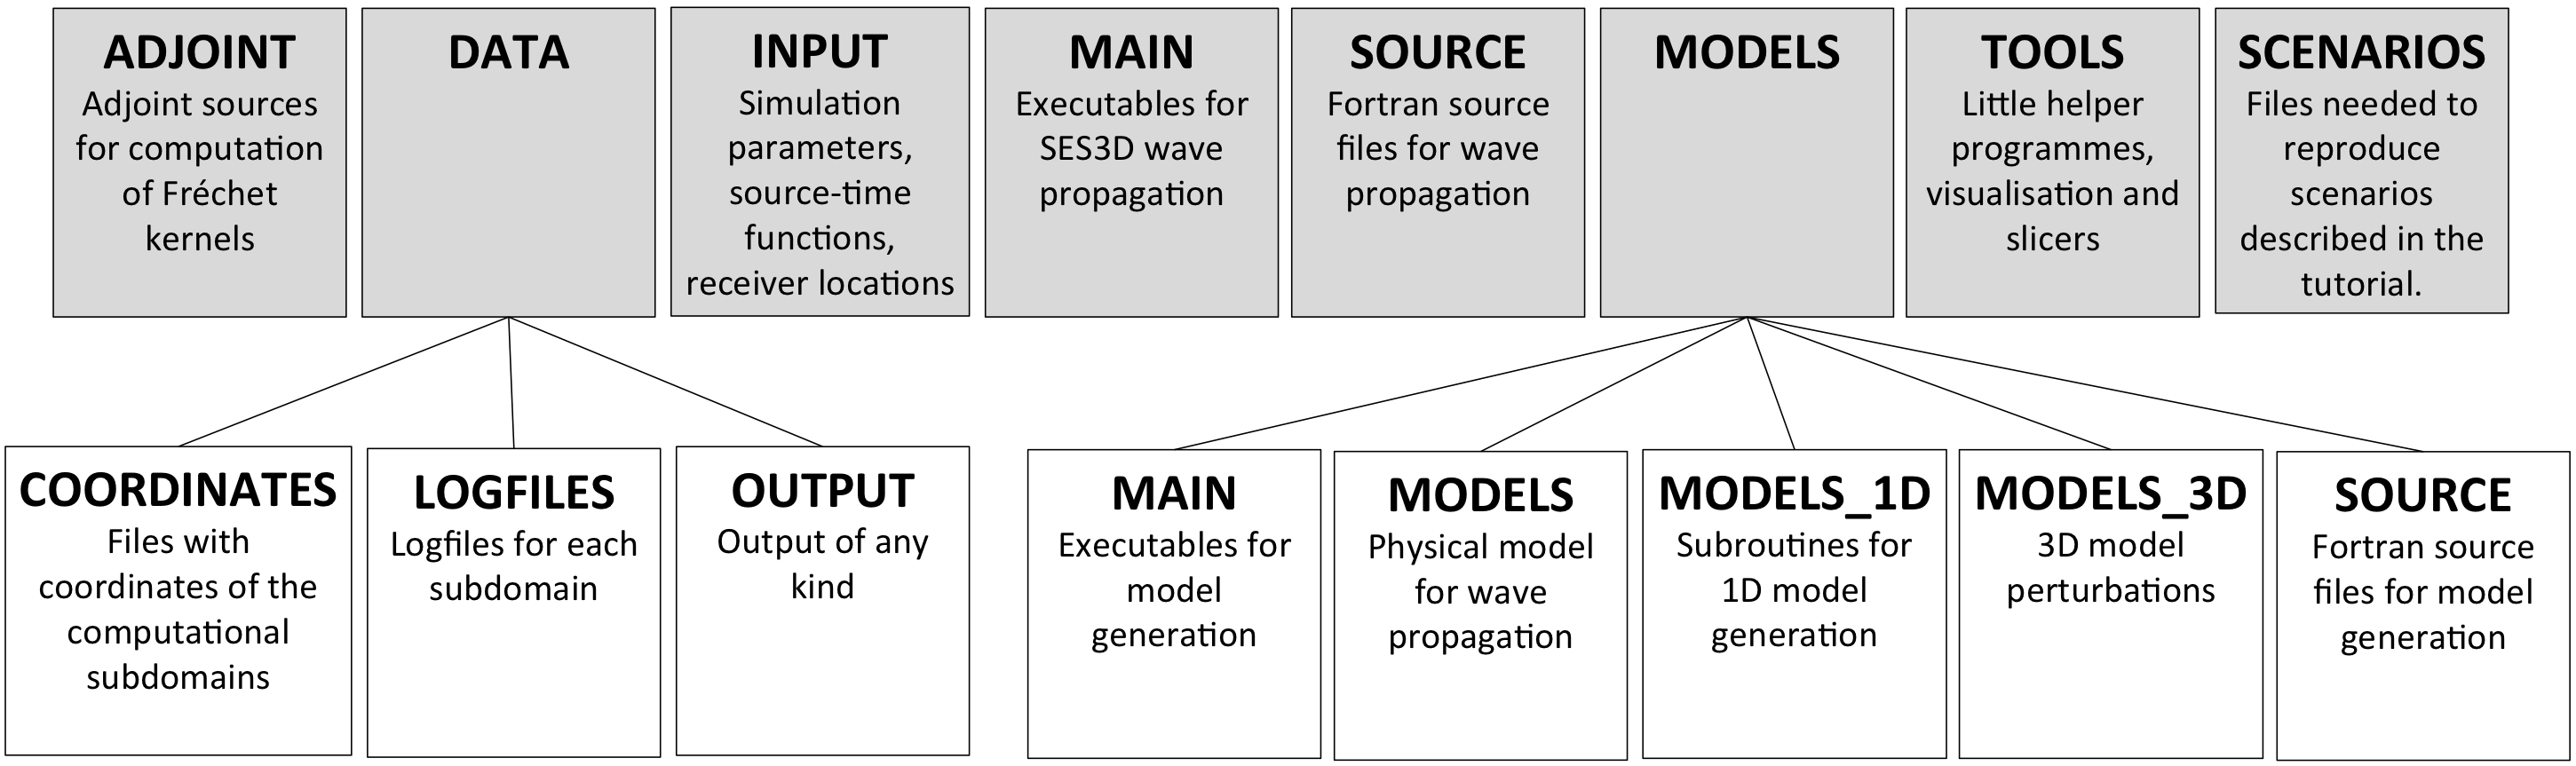
\includegraphics{Figures/directory_structure.png}}
\caption{\SES directory structure. See the text for detailed descriptions.}\label{F:directory_structure}
\end{figure}
\end{center}
%========================================================================

%====================================================================
% Source files.
%====================================================================

\section{Source files for wave propagation}

The principal source files for the wave propagation simulation and the computation of Fr\'{e}chet kernels can be found in the directory \texttt{SOURCE}. These are:\\[5pt]
\texttt{ses3d\_main.f90:} Initialisation of MPI, open logfiles, call subroutines for initialisation, call subroutines to iteratively advance the wavefield, monitor PML stability, write intermediate wave field in adjoint runs, clean up MPI and close files at the end of the iteration.\\[5pt]
\texttt{ses3d\_modules.f90:} Definition of variables and parameters.\\[5pt]
\texttt{ses3d\_input.f90:} Read parameter files \texttt{Par\_*}, read \texttt{boxfile} (contains information concerning the parallelisation), read 3D model parameters, read source time functions (\texttt{stf\_*}), read receiver locations (\texttt{recfile\_*}), read adjoint source locations (\texttt{ad\_srcfile}).\\[5pt]
\texttt{ses3d\_init.f90:} Set up grid point geometry, make mass matrix, compute receiver locations in unit cube coordinates, compute point source location in unit cube coordinates, read adjoint source
time functions, initialise PML damping profiles.\\[5pt]
\texttt{ses3d\_evolution.f90:} Propagate dynamic fields one time step forward.\\[5pt]
\texttt{ses3d\_grad.f90:} Compute Fr\'{e}chet kernels.\\[5pt]
\texttt{ses3d\_output.f90:} Collection of subroutines to write seismograms, store intermediate wave fields, write wave field snapshots and write Fr\'{e}chet kernels.\\[5pt]
\texttt{ses3d\_miscellaneous.f90:} Subroutines to add external forces (single force, moment tensor source, adjoint sources) and for the communication between compute cores.\\[5pt]
The above source files must be compiled together, e.g. by running the script \texttt{s\_make} located in the \texttt{SOURCE} directory. \textbf{A recompilation is necessary after a change of
the parallelisation scheme, i.e. a change of the division of the spherical section into subsections.}\\[5pt]
The script \texttt{s\_make} compiles all source files and combines them into the executables \texttt{ses3d.exe} located in the directory \texttt{MAIN}. Executing \texttt{ses3d.exe}
starts the forward or adjoint wave propagation.

%====================================================================
% Variable style.
%====================================================================

\section{Variable style and nomenclature of 3D fields}\label{S:variables}

In \SES, dynamics fields (velocity, stress, strain, material parameters, etc.) are implemented in the form of six-dimensional arrays. This is illustrated in figure \ref{F:variables} with the example of the
$\theta$-component velocity field. The first three dimensions of the array correspond to the element indices within a spherical subsection in $\theta$-, $\phi$- and radial directions. Note that
the radial index increases from the surface, where it is equal to $0$, towards greater depth. The last three indices are used to address the nodes within one element.\\[5pt]
Throughout \SES, $\theta$-components (colatitude) are labelled with \texttt{x}, $\phi$-components (longitude) with \texttt{y} and radial components with \texttt{z}. This is intended to keep the variable names short.
%========================================================================
\begin{center}
\begin{figure}
\center\scalebox{0.25}{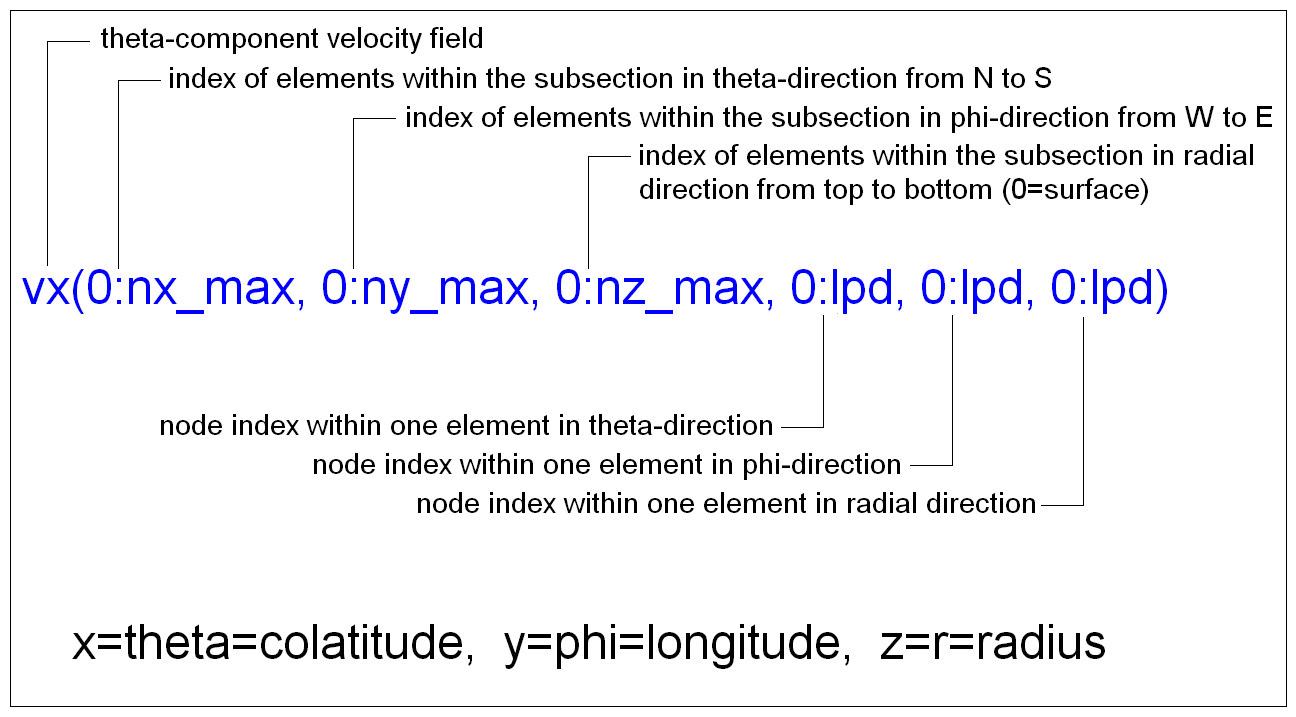
\includegraphics{Figures/variables.png}}
\caption{Structure and nomenclature of the dynamic fields in \SES. The example is for the velocity field in colatitudinal ($\theta$) direction.}\label{F:variables}
\end{figure}
\end{center}
%========================================================================

%====================================================================
% Calls to caution.
%====================================================================

\section{Calls to caution}\label{S:caution}

Each numerical method needs to be handled with care, and \SES is no exception. The following paragraphs are concerned with some of the difficulties that a user may encounter when working with \SES. It is generally recommended to assess the accuracy of numerical solutions by comparing them to semi-analytical solutions that exist for simplified models, e.g. radially symmetric Earth models.

\subsection{Absorbing boundaries}

\SES avoids unphysical reflections from the lateral and lower boundaries of the spherical section using a variant of the perfectly matched layers technique, called the method of anisotropic perfectly matched layers (APML, e.g. Teixeira \& Chew, 1997). It consists in the modification of the elastic wave equation within a narrow region along the unrealistic boundaries of the spherical section. The mathematical details of this method are explained in section \ref{S:absbound_theo}.\\[5pt]
The width of the absorbing boundary region, in terms of the number of elements, is specified by the parameter \texttt{pml} in the \texttt{ses3d\_modules.f90} source file. A good choice is \texttt{pml=3}, i.e. an absorbing boundary layer that is three elements wide.\\[5pt]
Within the absorbing layer, incoming waves are attenuated. This means that one should place neither receivers nor sources within the boundary layer. It is recommended to have at least two elements between the absorbing layer and receivers and sources.\\[5pt]
Contrary to what their name suggests, perfectly matched layers are not perfect. The imperfection comes in the form of two undesirable phenomena: (1) Incident waves are not completely absorbed by the absorbing layers. This means that small unphysical reflections will always be present. These can be minimised by placing sources and receivers further away from the boundaries. (2) All variants of the perfectly matched layers technique are long-term unstable. This means that the wavefield amplitudes may grow indefinitely for very long simulations, where the term \emph{very long} is not very well defined. 

\subsection{Seismic discontinuities and the crust}\label{S:crust}

Realistic Earth models typically contain discontinuities. Spectral-element solutions are correct only when discontinuities coincide with the edges of elements, such that the shared boundary
nodes take the different values from each side of the discontinuity. The inflexible grid of \SES is not always capable of accounting for discontinuities in the exact way. This means that discontinuities of the material properties may be located in the interior of elements. As a result, the numerical solutions may not be as exact as they would be in the case of perfectly honoured discontinuities. This effect is difficult to quantify, and it mostly concerns surface waves.\\[5pt]
A related problem is the implementation of thin crustal layers that may be thinner than a layer of elements. This can also produce inaccurate numerical solutions.\\[5pt]
Difficulties with thin crustal layers and discontinuities can most easily be avoided by the implementation of long wavelength equivalent models (e.g. Capdeville \& Marigo, 2007, 2008; \href{http://www.geo.uu.nl/~fichtner/papers/2008_fichtner_DCM.pdf}{Fichtner \& Igel, 2008}).

\subsection{The poles and the core}

Since \SES operates in the natural spherical coordinate system, one must exclude the poles and the core from the computational domain. A the centre of the Earth, spatial derivatives in spherical coordinates are singular. Also, the elements become very small near the poles and near the core, so that the time step \texttt{dt} must be chosen very small. To run \SES efficiently, the spherical sections should not be deeper than $\sim 3000$ km and not closer than $\sim 20^\circ$ to one of the poles.                  
	\chapter{Scenarios}

The practical part of this tutorial is built around realistic scenarios that introduce various aspects of \SES, ranging from basic the input to the implementation of 3D models, the compuation of sensitivity kernels, and rotations of the computational domain. For each of the scenarios, various source and input files must be changed. Those files can be found in the \texttt{SCENARIOS} folder.

%====================================================================
% Anatolia
%====================================================================

\section{Regional-scale wave propagation: Anatolia}\label{S:Anatolia}

In our first scenario, we work with an earthquake that occurred on August 25, 2007 in eastern Turkey. The hypocentre location is: latitude: $39.26^\circ$, longitude: $41.04^\circ$, depth: $5.0$ km. Our goal is to introduce the input files of \SES, implement a 3D heterogeneous model, and compute sensitivity kernels.\\[5pt]
The default setup of \SES is made to fully reproduce this example. All input and source files that are specific to this scenario can also be found in the \texttt{SCENARIOS/ANATOLIA/} folder.

%- Input ===============================================================

\subsection{Input}

\subsubsection{Model setup}\label{S:model_setup}

The geometrical setup of the model is described in the file \texttt{setup} in the directory \texttt{INPUT}. In our specific example, the computational domain ranges from $47.1^\circ - 55.9^\circ$ colatitude (colatitude$=90^\circ -$latitude), from $23.1^\circ - 42.9^\circ$ longitude, and from a radius of $5,900,000.0 - 6,371,000.0$ m, i.e. from $471$ km depth to the surface of the Earth. For the moment, we ignore visco-elastic dissipation (\texttt{is\_diss=0}), and we construct a homogeneous model where all velocities and density are set to zero (\texttt{model\_type=1}). More on the generation of specific Earth models can be found in section \ref{S:model_generation}.\\[5pt]
We parallelise the computations by dividing the computational domain into $3$ subdomains in colatitudinal direction (\texttt{px}=3), $4$ subdomains in longitudinal direction (\texttt{py}=4) and $4$ subdomains in depth direction (\texttt{pz}=4). Thus, we have a total of $48$ subdomains, each of which is assigned to one compute core. The parallelisation in \SES is shown schematically in figure \ref{F:parallel}.\\[5pt]
Within each of the subdomains, the finite elements are numbered from $0$ to $66$/\texttt{px}$=22$ in colatitudinal direction (\texttt{nx\_global=66}), from $0$ to $108$/\texttt{py}$=27$ in longitudinal direction (\texttt{ny\_global=108}), and from $0$ to $28$/\texttt{pz}$=7$ in radial direction (\texttt{nz\_global=28}). The total number of elements in the complete computational domain is (\texttt{nx\_global}+\texttt{px})(\texttt{ny\_global}+\texttt{py})(\texttt{nz\_global}+\texttt{pz})$=247,296$. Note that the ratios\\[5pt]
\texttt{nx\_max}=\texttt{nx\_global}/\texttt{px}, \texttt{ny\_max}=\texttt{ny\_global}/\texttt{py} and \texttt{nz\_max}=\texttt{nz\_global}/\texttt{pz}\\[5pt]
must all be integers. The values of \texttt{nx\_max}, \texttt{ny\_max} and \texttt{nz\_max} must be set in the first lines of the source file \texttt{ses3d\_modules.f90} in the directory \texttt{SOURCE}, \textbf{and the code must be recompiled after changing these numbers.}\\[5pt]
Within each element, the dynamic fields (e.g. stress tensor, displacement field, ...) are represented by Lagrange polynomials of degree $4$ (\texttt{lpd}=4). One element therefore comprises $(4+1)^3=125$ grid points, meaning that the complete computational domain contains $247,296 \cdot 125 = 30,912,000$ grid points.\\[5pt]
For the moment, we perform a pure forward simulation, and therefore set the parameter \texttt{adjoint\_flag} to $0$. The remaining parameters in the \texttt{setup} file, as well as the actual meaning of the  \texttt{adjoint\_flag} will be discussed in section \ref{S:kernels}.
%====================================================================
\begin{center}
\begin{figure}
\center\scalebox{0.37}{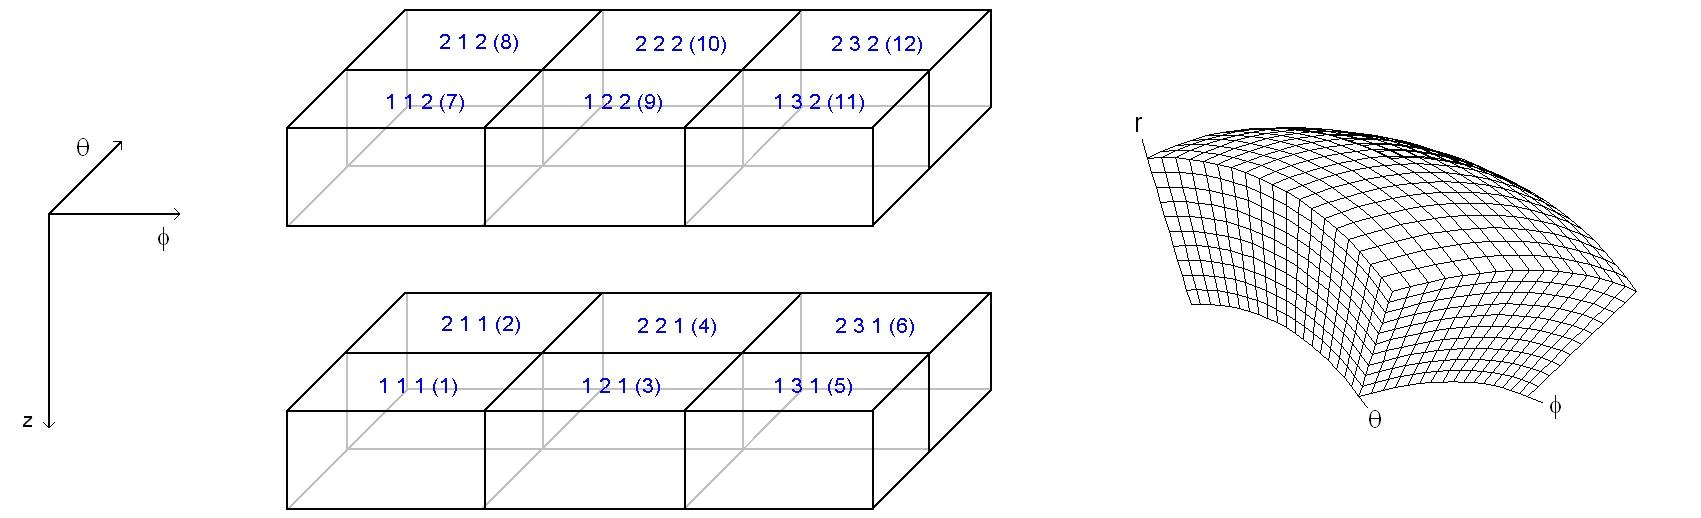
\includegraphics{Figures/parallel_boxes.jpg}} 
\caption{Schematic representation of the parallelisation of \SES. The spherical section is subdivided into subsections, and each subsection is assigned to one compute core. A triple index and a single index (in parenthesis) is assigned to a subsection.}\label{F:parallel}
\end{figure}
\end{center}
%====================================================================

\subsubsection{Event information}

\SES can model a sequence of earthquakes (events), each labelled by an integer number. The event information for the event numbered $x$ is contained in the file \texttt{event\_x}. A list of all events to be modelled must be provided in the file \texttt{event\_list} (number of events followed by their label).\\[5pt]
In this example, we label our event with $1$. The event information in the file \texttt{event\_1} are the colatitude (\texttt{xxs}$=50.740^\circ$), longitude (\texttt{yys}$=41.040^\circ$) and depth (\texttt{zzs}$=5,000$ m) of the source. The source type (\texttt{srctype}) is set to $3$, which indicates a moment tensor source. (The options \texttt{srctype}=$1,2,3$ correspond to vector forces in the colatitudinal, longitudinal and radial directions, respectively.) The moment tensor in our simulation corresponds to an explosion:
\begin{equation}
\w{M}=\begin{pmatrix}
M_{\theta\theta} & M_{\theta\phi} & M_{\theta r} \\
M_{\theta\phi} & M_{\phi\phi} & M_{\phi r} \\
M_{\theta r} & M_{\phi r} & M_{ r r}
\end{pmatrix}
=
\begin{pmatrix}
1.0 & 0.0 & 0.0 \\
0.0 & 1.0 & 0.0 \\
0.0 & 0.0 & 1.0
\end{pmatrix}\, \cdot 10^{16}\,\text{N\,m}\,.
\end{equation}
In our simulation we perform \texttt{nt}$=4,000$ time steps, each of which is \texttt{dt}$=0.13$ s long. As output directory for the synthetic seismograms we set \texttt{../DATA/OUTPUT/1.8s/}.

\subsubsection{Receiver locations}

A list of receivers must be provided in the file \texttt{recfile\_*} located in the \texttt{INPUT} directory. The * is to be replaced by the event number, i.e. we have \texttt{recfile\_1} in our case. Following the number of receivers in the list, each receiver is listed with its name and, in the line below, colatitude ($^\circ$), longitude ($^\circ$) and depth (m). The depth must be larger or equal to zero, i.e., no receivers are allowed above the surface. Each receiver name is exactly $12$ characters long. These characters are typically occupied by the actual station name, the network and any type of additional information.

\subsubsection{Source time function}

The source time function \texttt{stf} is given in the \texttt{INPUT} directory in the form of an ASCII list. Each entry is a sample of the source time function, and the time spacing must equal the one in the \texttt{event\_*} files. (This time spacing is not given explicity in \texttt{stf}. In our case it is \texttt{dt}$=0.13$ s.)\\[5pt]
The source time function should ideally be a bandpass filtered Heaviside function. Periods that are too long cannot be modelled because the computational domain is finite, and periods that are too short cannot be modelled accurately because of discretisation errors. (Furthermore, short periods tend to produce artefacts when they interact with the absorbing boundaries.) As a rule of thumb, the shortest period in the source time function should be such that the corresponding wavelength is not shorter than $1.5$ to $2$ elements. In our case, one element is around $14$ km wide (e.g. $69$ elements over a distance of $55.9^\circ-47.1^\circ=8.8^\circ$), meaning that the minimum wavelength should be $21$ to $28$ km. Assuming a minimum propagation velocity of around $3$ km$/$s, this translates to a minimum period of $7$ to $9$ s. For our example we use a Heaviside function filtered between $8$ s and $100$ s (see figure \ref{F:stf}).
%====================================================================
\begin{center}
\begin{figure}
\center\scalebox{0.30}{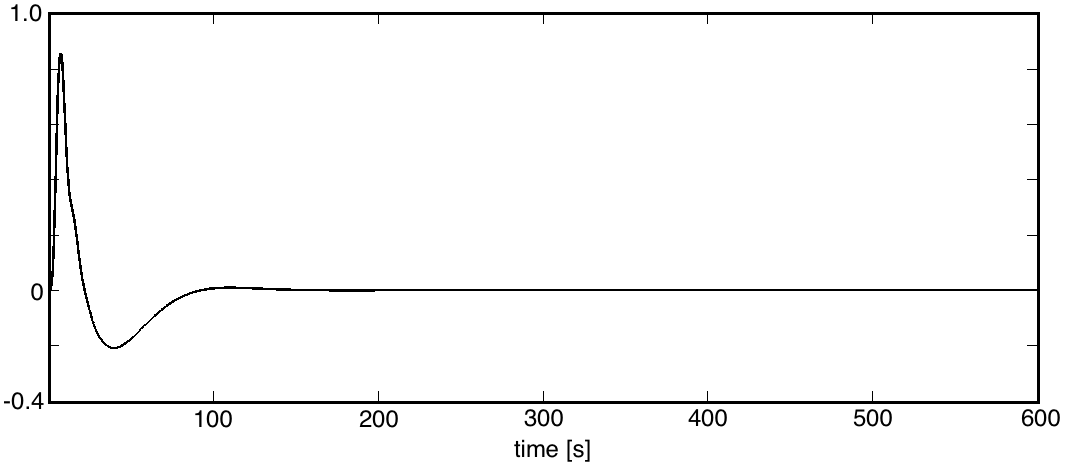
\includegraphics{Figures/stf.png}} 
\caption{Source time function. We use a Heaviside function bandpass filtered between $8$ s and $100$ s. The number of samples in the source time function file \texttt{stf} must be at least the number of time steps \texttt{nt} given in the event files \texttt{event\_*}.}\label{F:stf}
\end{figure}
\end{center}
%====================================================================


%====================================================================
% Model generation
%====================================================================

\subsection{Model construction}\label{S:model_generation}

The construction of 3D Earth models in \SES is proceeds in two steps: (1) The construction of a 1D, i.e. radially symmetric, Earth model, and (2) the addition of 3D perturbations to the 1D model. To facilitate the solution of tomographic inverse problems, model construction in \SES is completely decoupled from the actual wave propagation. The necessary executables can be generated by compiling the source code located in \texttt{MODELS/SOURCE}, e.g. by running the script \texttt{s\_make}. The executables are located in \texttt{MODELS/MAIN}.

\subsubsection{Step 1: Constructing 1D Earth models}

We construct 1D Earth models by running \texttt{generate\_models.exe}, located in \texttt{MODELS/MAIN}. This programme reads the geometrical setup provided in the \texttt{setup} file. The type of 1D Earth model is specified by the parameter \texttt{model\_type} in the \texttt{setup} file. In our case, \texttt{model\_type}$=1$, which generates a homogeneous model with all velocities and density set to zero.\\[5pt]
The following alternative Earth models are currently implemented:
\begin{enumerate}
\item \texttt{model\_type=2}: Isotropic version of PREM (Dziewonski and Anderson, 1981).
\item \texttt{model\_type=3}: All-zero elastic model with a smoothed version of the Q model QL6 (Durek \& Ekstr\"{o}m).
\item \texttt{model\_type=4}: Modified version of the isotropic PREM with the 220 km discontinuity replaced by a linear gradient.
\item \texttt{model\_type=7}: AK135 (Kennett et al., 1995).
\end{enumerate}
The detailed setups of these 1D model can be found in \texttt{MODELS/MODELS\_1D}.\\[5pt]
Running \texttt{generate\_models.exe} produces files containing the physical model parameters ($\lambda, \mu, A, B, C$ and $1/\rho$) for each of the computational subdomains ($48$ in our case). These are located in \texttt{MODELS/MODELS}. Furthermore, \texttt{generate\_models.exe} writes the \texttt{boxfile} which summarises the geometrical setup and the parallelisation of the computational domain. All these files serve as input for the actual wave propagation.\\[5pt]
For debugging purposes, \texttt{generate\_models.exe} also writes human-readable vertical profiles through each of the subdomains. These are named \texttt{prof\_*}, where * denotes the index of the subdomain.

\subsubsection{Step 2: Adding 3D heterogeneity}

\paragraph{Description of 3D heterogeneous models}\label{S:3Dmodels}

Following the construction of a 1D model, we add 3D perturbations, located in \texttt{MODELS/MODELS\_3D}. The term \emph{3D perturbations} is loosely defined. In our specific case where the 1D model is the homogeneous model with all parameters set to zero, the perturbations are in fact the absolute 3D model itself.\\[5pt]
The 3D perturbations of P velocity (in km$/$s, file \texttt{dvp}), SH velocity (in km$/$s, file \texttt{dvsh}), SV velocity (in km$/$s, file \texttt{dvsv}) and density (in g$/$cm$^3$, file \texttt{drho}) are parametrised in discrete regular blocks. The geometry of the blocks, i.e. the locations of their bounding grid points, is descibed in the files \texttt{block\_x} (colatitudinal direction), \texttt{block\_y} (longitudinal direction) and \texttt{block\_z} (radial direction).\\[5pt]
In our specific example, the horizontal grid spacing is $0.25^\circ$ from $5871$ km to $6266$ km radius, and $0.1^\circ$ from $6266$ km to $6371$ km radius. The radial grid spacing is $5$ km throughout the model. This variable grid spacing roughly reflects the tomographic resolution that we expect in different depth ranges. Figure \ref{F:block_files} illustrates how the variable grid spacing within the two subdomains is represented in the \texttt{block\_*} files. A schematic representation of the grid spacing is shown in figure \ref{F:geometry}.\\[5pt]
Note that the grid on which the 3D model is described, is completely independent of the numerical grid used in the wave propagation machinery or for the generation of the 1D model. This independence allows us to add 3D model perturbations to any previously constructed 1D model - regardless of its specific setup.\\[5pt]
The files containing the actual model perturbations (\texttt{dvp, dvsh, dvsv, drho}) are organised as shown in figure \ref{F:perturbations}. Note that the velocity and density values are given for the volumetric blocks bounded by the grid points. The number of blocks is therefore smaller than the number of grid points.
%====================================================================
\begin{center}
\begin{figure}
\center\scalebox{0.35}{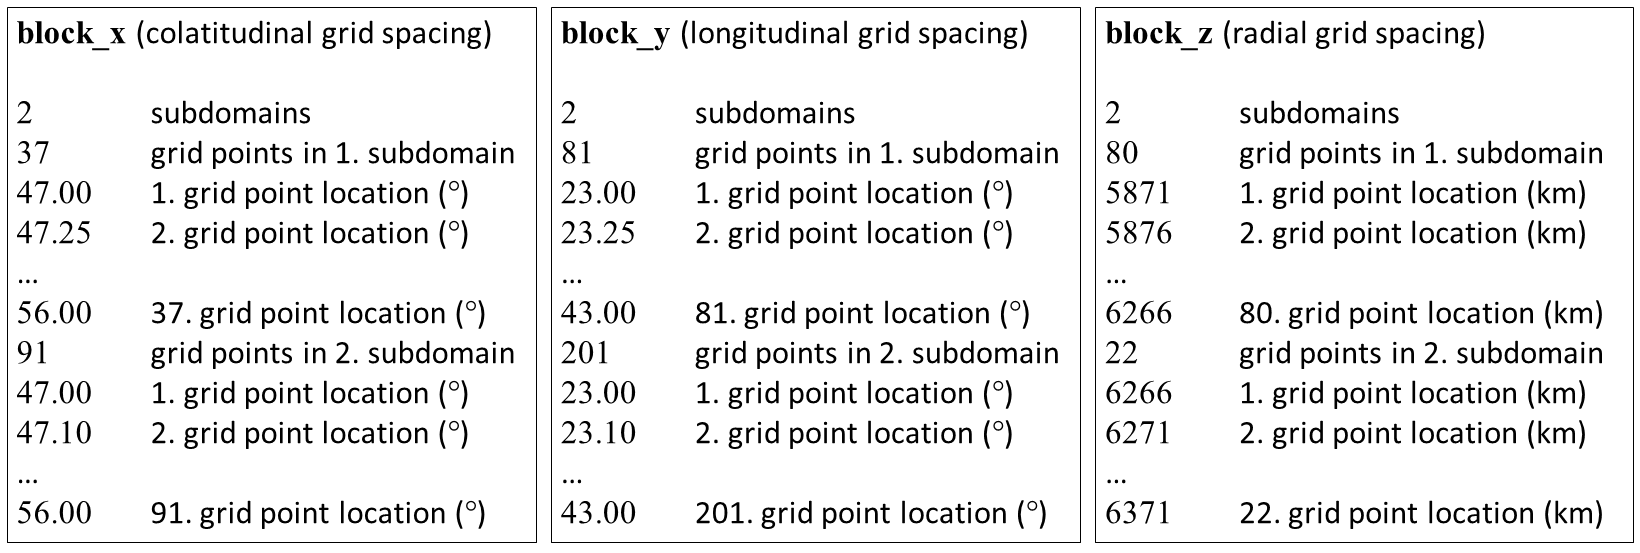
\includegraphics{Figures/block_files.png}} 
\caption{Organisation of the \texttt{block\_*} files that describe the geometric parametrisation of the 3D heterogeneities.}\label{F:block_files}
\end{figure}
\end{center}
%====================================================================
%====================================================================
\begin{center}
\begin{figure}
\center\scalebox{0.35}{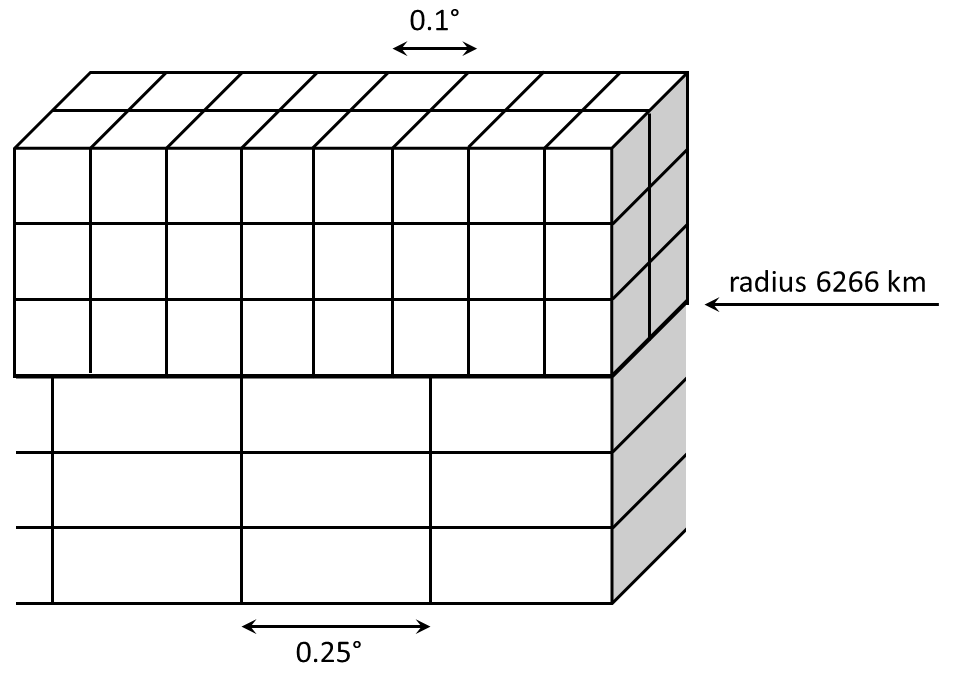
\includegraphics{Figures/geometry.png}} 
\caption{Schematic representation of the variable grid spacing of the 3D heterogeneities. Above a radius of $6266$ km, the horizontal grid spacing is $0.1^\circ$. Below, it is $0.25^\circ$.}\label{F:geometry}
\end{figure}
\end{center}
%====================================================================
%====================================================================
\begin{center}
\begin{figure}
\center\scalebox{0.35}{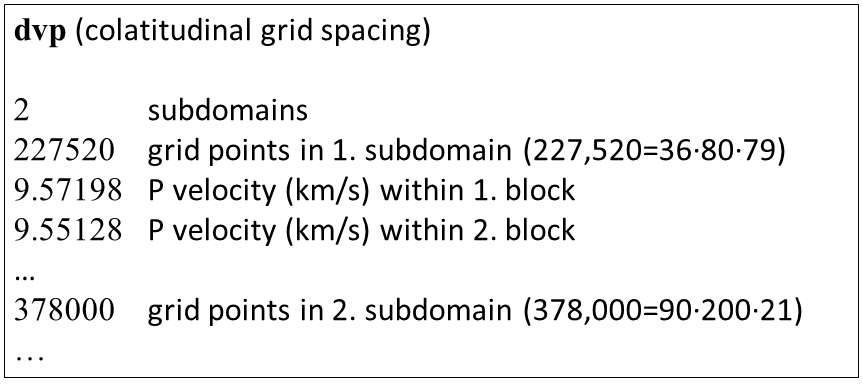
\includegraphics{Figures/perturbations.png}} 
\caption{Organisation of the P velocity perturbations in the file \texttt{dvp}. The number of subdomains ($2$) is followed by the number of blocks in the first subdomain ($227,520$). The actual values of P velocity (perturbations) are given as a list that results from looping over the 3D volume. The outer loop if over colatitude, the intermediate loop over longitude, and the inner loop over radius. This list is then followed by a similar list for the second subvolume. The files \texttt{dvsh}, \texttt{dvsv} and \texttt{drho} are organised analogously.}\label{F:perturbations}
\end{figure}
\end{center}
%====================================================================

\paragraph{Adding 3D heterogeneity to the 1D model}

We can add 3D perturbations in $\vp$, $\vsv$, $\vsh$ and $\rho$ by running the executable \texttt{add\_perturbation.exe}, located in \texttt{MODELS/MAIN}. Using geometric information from the \texttt{setup} file and the \texttt{boxfile}, the programme \texttt{add\_perturbation.exe} reads \texttt{dvp}, \texttt{dvsv}, \texttt{dvsh} and \texttt{drho} and add these 3D perturbations to the pre-existing model files in \texttt{MODELS/MODELS}. For our example we use a 3D model of the Anatolian region, described in \href{http://www.geo.uu.nl/~fichtner/papers/2013_Fichtner_EPSL.pdf} {Fichtner et al., 2013a} and \href{http://www.geo.uu.nl/~fichtner/papers/2013_Fichtner_GJI.pdf}{Fichtner et al., 2013b}. The $\vsv$ distribution in this model is shown in figure \ref{F:anatolia}. 
%====================================================================
\begin{center}
\begin{figure}
\center\scalebox{0.37}{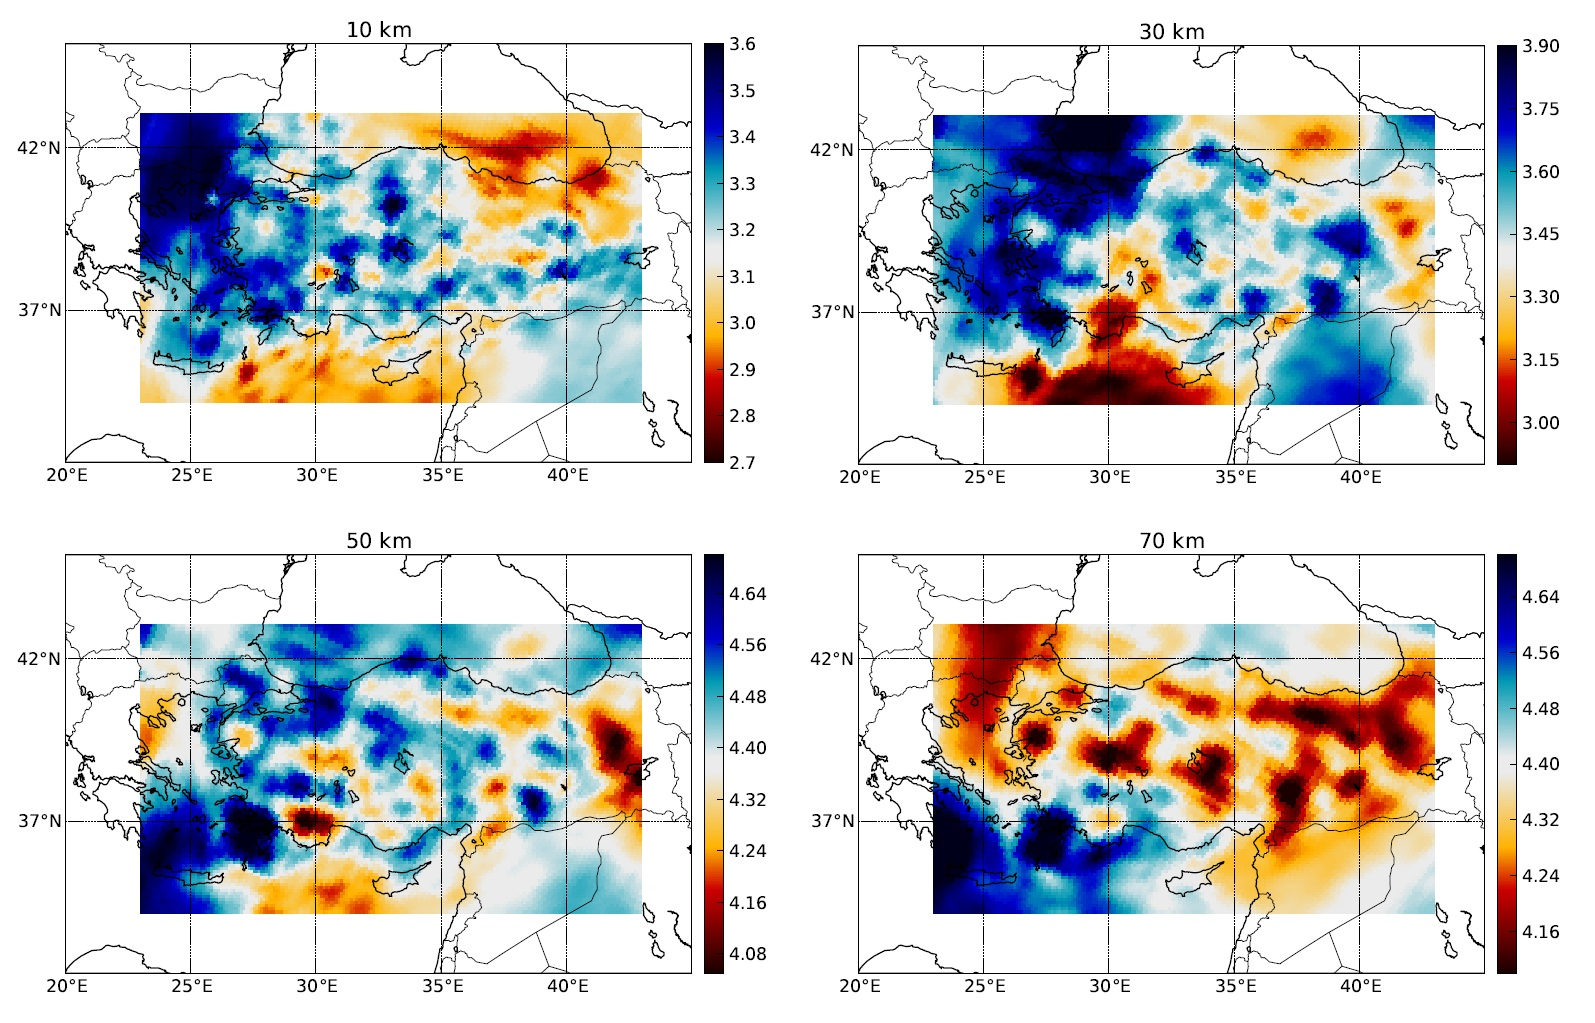
\includegraphics{Figures/anatolia.jpg}} 
\caption{Distribution of $\vsv$ in the Anatolian model at $20$ km, $50$ km and $100$ km depth. The depth slices in this figure were generated using the Python tool \texttt{models.py} in the \texttt{TOOLS} directory.}\label{F:anatolia}
\end{figure}
\end{center}
%====================================================================

%====================================================================
% Output
%====================================================================

\subsection{Simulation of wave propagation and output}

The actual wave propagation executable is \texttt{ses3d.exe}, located in \texttt{MAIN}. Upon running \texttt{ses3d.exe}, the geometrical information in \texttt{setup}, the event information in \texttt{event\_x} and \texttt{event\_list}, as well as the physical model parameters in \texttt{MODELS/MODELS} are read. The seismic wavefield is the propagated forward in time, for \texttt{nt} time steps. After the last time step, synthetic seismograms are written to the output directory, in our case \texttt{DATA/OUTPUT/1.8s/}. The three-component synthetic seismograms for station BALB are shown in figure \ref{F:seismograms}.
%====================================================================
\begin{center}
\begin{figure}
\center\scalebox{0.47}{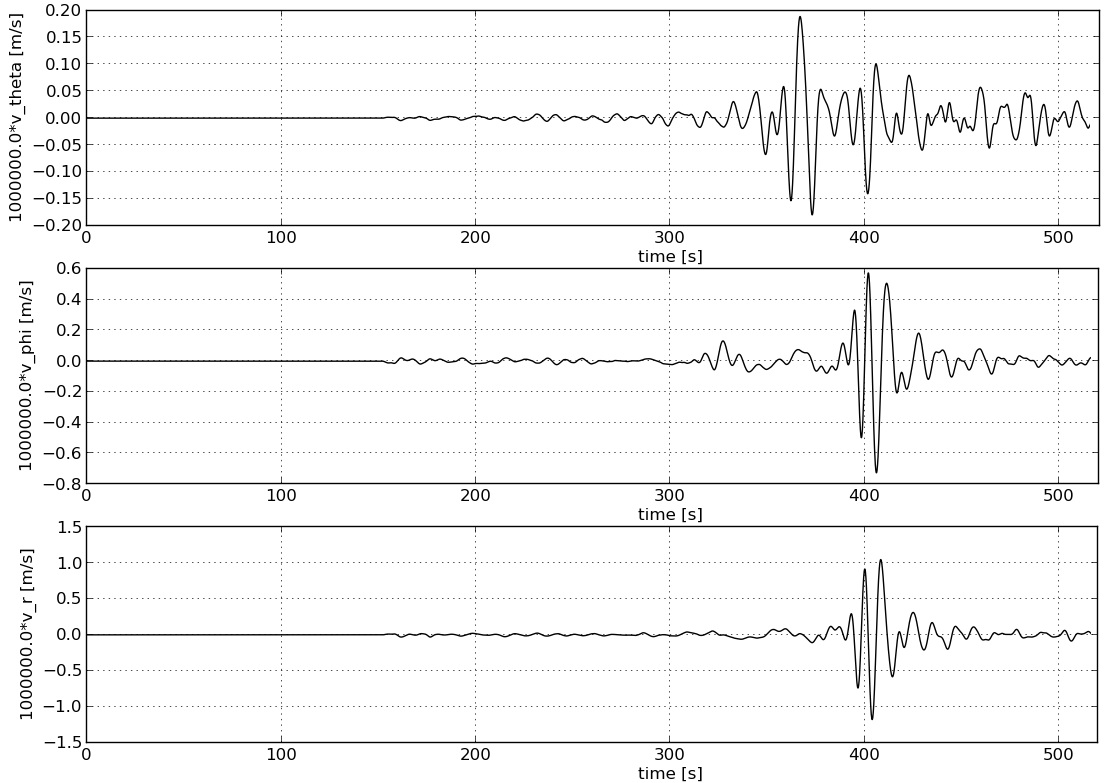
\includegraphics{Figures/seismograms.jpg}} 
\caption{Three-component synthetic seismograms for station BALB.}\label{F:seismograms}
\end{figure}
\end{center}
%====================================================================

%====================================================================
% Computing sensitivity kernels
%====================================================================

\subsection{Computing sensitivity kernels}\label{S:kernels}

The computation of sensitivity kernels proceeds in several steps. First of all, a forward simulation must be run with the \texttt{adjoint\_flag} in the \texttt{setup} file set to \texttt{1}. This ensures that the forward field is stored in the directory which appears in the last line of the \texttt{setup} file. Make sure enough storage is actually available.\\
One the forward field is computed, adjoint sources for a variety of measurements can be computed using Python tools in the \texttt{TOOLS} directory. An example of this procedure is given below:\\[5pt]
\texttt{run seismograms.py}: Compile Python tool for reading and plotting seismograms.\\[5pt]
\texttt{run adjoint\_source.py}: Compile Python tool for the computation of adjoint sources.\\[5pt]
\texttt{s=ses3d\_seismogram()}: Make empty seismogram structure.\\[5pt]
\texttt{s.read('../DATA/OUTPUT/1.8s/','BALB\_.KO.\_\_\_')}: Read seismograms for station BALB.\\[5pt]
\texttt{s.plot(1e6)}: Plot seismograms, scaled by a factor of $1\cdot 10^6$.\\[5pt]
\texttt{a=adjoint\_source()}: Make empty adjoint source structure.\\[5pt]
\texttt{a.fetch\_seismogram(s)}: Load seismograms into the adjoint source structure.\\[5pt]
\texttt{a.make\_adsrc\_mttime('z',391.0,412.0,0.1,True)}: Compute adjoint source for a multitaper measurement of a time delay on the vertical component for the window from $391.0$ s to $412.0$ s at the frequency of $0.1$ Hz.\\[5pt]
\texttt{a.plot()}: Plot adjoint source.\\[5pt]
\texttt{a.write('../ADJOINT/1/','ad\_src\_1')}: Write adjoint source to file.\\[5pt]
It is important that the adjoint sources for \texttt{event\_1} are written to the directory \texttt{ADJOINT/1/}. For an event with event file \texttt{event\_102}, the adjoint sources would be expected to be located in \texttt{ADJOINT/102/}.\\
For each event, multiple adjoint sources may be computed. In our example, we use only one. The second adjoint source time function would be named \texttt{ad\_src\_2}, and it would be located in the same directory. The file \texttt{ad\_srcfile} contains a list of all adjoint source time functions used for this specific event. In our case, \texttt{ad\_srcfile} contains only 2 lines:\\[7pt]
\texttt{1} (indicates that one adjoint source is used)\\
\texttt{50.36 27.88 1000.0} (colatitude, longitude and depth of the adjoint source)\\[7pt]
Once the adjoint sources are computed, simply set the \texttt{adjoint\_flag} to \texttt{2} and re-run the wave propagation code. Sensitivity kernels will then be computed automatically, and stored in the output directory specified in the event file. Then, using \texttt{project\_kernels.exe} in the \texttt{TOOLS} directory, the kernels can be projected onto the grid used to represent 3D models. This is particularly helpful in the context of tomographic inverse problems, but also for plotting purposes. Since the projected kernels have the same format as a 3D model, we can use the Python tool \texttt{models.py} to read and plot the projected kernels. The result is shown in figure \ref{F:kernel}.
%====================================================================
\begin{center}
\begin{figure}
\center\scalebox{0.35}{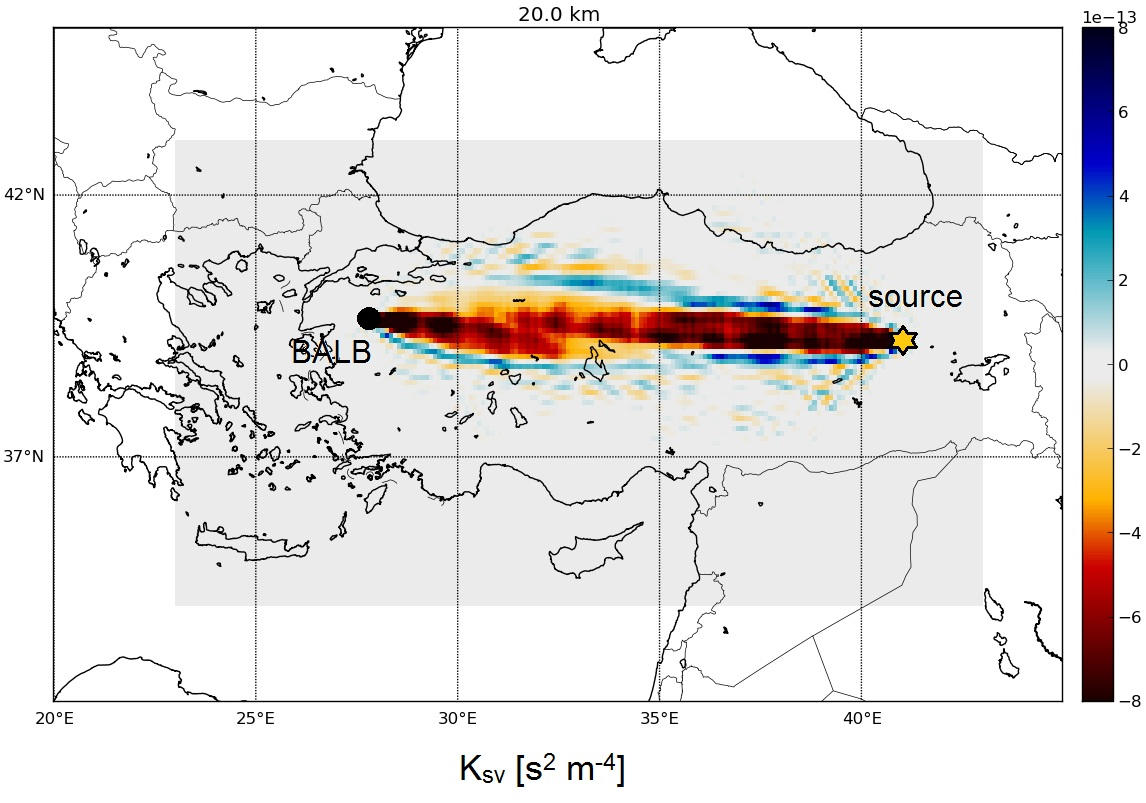
\includegraphics{Figures/kernel.jpg}} 
\caption{Sensitivity kernel with respect to the SV velocity at $20$ km depth. The measurement is  a multitaper measurement of a time delay on the vertical component of station BALB for the window from $391.0$ s to $412.0$ s at the frequency of $0.1$ Hz.}\label{F:kernel}
\end{figure}
\end{center}
%====================================================================

%====================================================================
% North America
%====================================================================

\section{Continental-scale wave propagation: North America}\label{S:North_America}

Seismic wave propagation in \SES may become inefficient when the computational domain is too close to the poles where the elements become very small, thus enforcing a small time step. This problem is particularly relevant for large domains that approach or even include the poles. To avoid excessively small time steps, the computational domain can be rotated away from the poles towards the equator.\\[5pt]
This rotation procedure will play a central role in the following scenario where we consider seismic wave propagation across North America and the North Atlantic. The scenario-specific input and source files are located in the directory \texttt{SCENARIOS/NORTH\_AMERICA}.

%====================================================================
% Rotating the computational domain.
%====================================================================

\subsection{Rotating the computational domain}

We are interested in the computational domain shown in figure \ref{F:NA1} that covers the North American continent and the North Atlantic. Since the domain closely approaches the North pole, where elements become very small, it should ideally be rotated southwards to avoid excessively small time steps. In this example, we rotate the complete domain southwards by $30^\circ$ around an axis given in terms of the unit vector
\begin{equation}
\w{n} = \left( \begin{array}{c} \text{cos}(40^\circ) \\ \text{sin}(40^\circ) \\ 0.0 \end{array} \right)
\end{equation}
The rotated domain is shown in figure \ref{F:NA2}. In rotated coordinates, the computational domain falls between the following colatitudes and longitudes that are specified in the \texttt{setup} file: \texttt{theta\_min=45.2}, \texttt{theta\_max=114.8}, \texttt{phi\_min=-119.8}, \texttt{phi\_max=-0.2}.\\[5pt]
Since the actual computations are not performed in the true physical but in the rotated domain, various input parameters must be adapted. The input parameters include the station and event coordinates, as well as the moment tensor. Python tools for the rotation of source/receiver locations and moment tensors can be found in \texttt{TOOLS/rotation.py}. These tools are also described in section \ref{S:Python}. While the original epicentral coordinates of our event are $\theta=34.08^\circ$, $\phi=-17.80^\circ$, the rotated cooridnates are $\theta'=61.30^\circ$, $\phi'=-30.10^\circ$. Similarly the moment tensor is rotated as follows:
\begin{align}
\w{M}&=\left(\begin{array}{ccc}
M_{tt} & M_{tp} & M_{tr} \\ M_{tp} & M_{pp} & M_{pr} \\ M_{tr} & M_{pr} & M_{rr}
\end{array}\right)
=
\left(\begin{array}{ccc}
-3.794 & 1.978 & -1.145 \\ 1.977 & 4.004 & -0.514 \\ -1.145 & -0.514 & -0.211
\end{array}\right) \notag\\
\to \notag \\
\w{M'}&=\left(\begin{array}{ccc}
M'_{tt} & M'_{tp} & M'_{tr} \\ M'_{tp} & M'_{pp} & M'_{pr} \\ M'_{tr} & M'_{pr} & M'_{rr}
\end{array}\right)
=
\left(\begin{array}{ccc}
-4.220 & -0.644 & -0.935 \\ -0.644 & 4.430 & -0.838 \\ -0.935 & -0.838 & -0.211
\end{array}\right) 
\end{align}
The rotated event parameters are specified in \texttt{event\_1}.\\[5pt]
Most plotting routines for models and seismograms that are located in the \texttt{TOOLS} directory, correctly account for the rotation. All that needs to be done is to set the rotation vector and the rotation angle in the file \texttt{TOOLS/rotation\_parameters.txt}.

%====================================================================
\begin{center}
\begin{figure}
\center\scalebox{0.45}{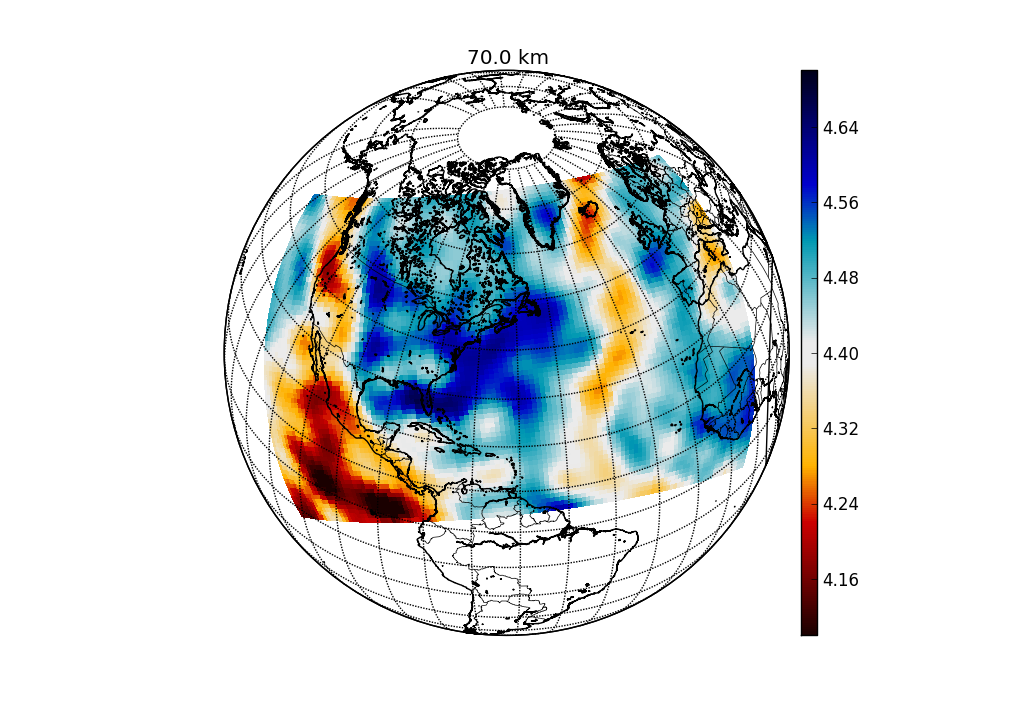
\includegraphics{Figures/NA1.png}} 
\caption{Horizontal slice through the SV velocity in model S40RTS (Ritsema et al., 2011) at $70$ km depth beneath North America and the North Atlantic. The computational domain approaches the North pole, and therefore needs to be rotated southwards. This plot was made with the tools provided in \texttt{TOOLS/models.py}.}\label{F:NA1}
\end{figure}
\end{center}
%====================================================================

%====================================================================
\begin{center}
\begin{figure}
\center\scalebox{0.45}{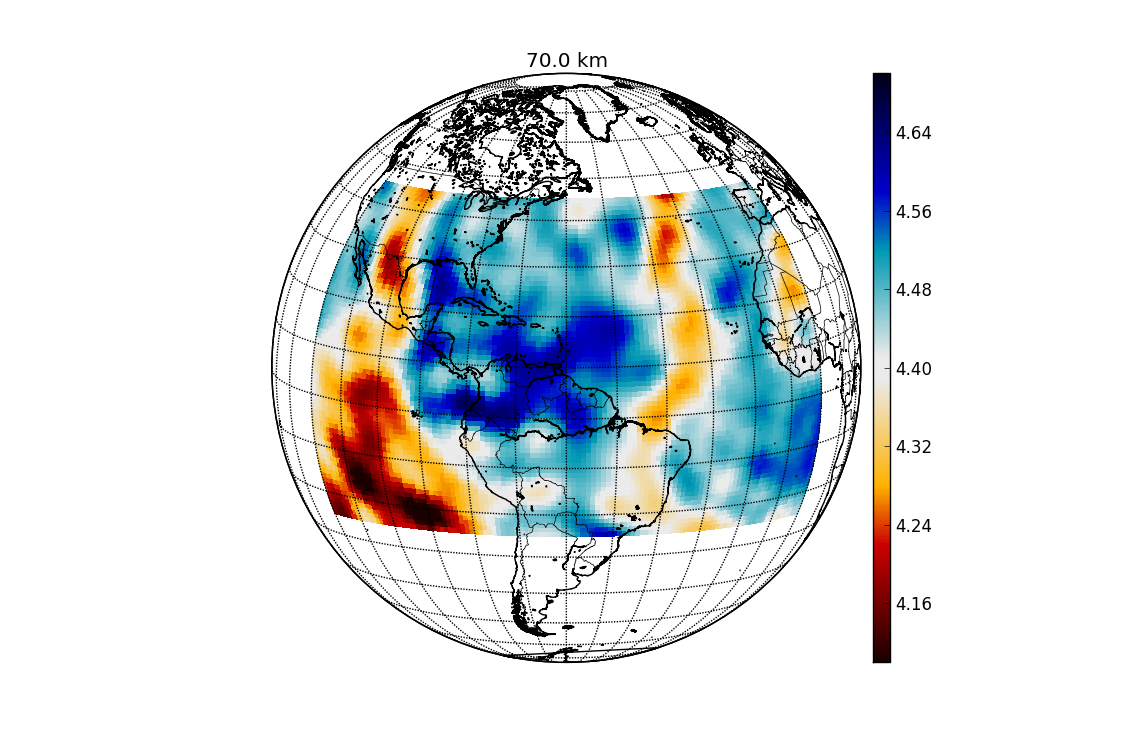
\includegraphics{Figures/NA2.png}} 
\caption{Rotated North America model. All computations are performed in this rotated domain. This plot was made with the tools provided in \texttt{TOOLS/models.py}.}\label{F:NA2}
\end{figure}
\end{center}
%====================================================================

\subsection{Source time function}\label{S:stf_NA}

While the computational domain in this scenario is comparatively large, its discretisation with $\sim 1.8$ elements per degree (specified in the \texttt{setup} file) is rather coarse. We are thus limited to the modelling of long-period wave propagation. To construct a suitable source time function, we can make use of the \texttt{make\_stf.py} scripts in the \texttt{TOOLS} directory. The function call\\[5pt]
\texttt{make\_stf(0.2,12000,1.0/200.0,1.0/100.0,'../INPUT/stf')}\\[5pt]
Produces a source time function that is a bandpass-filtered Heaviside function with cutoffs at $1/200$ Hz and $1/100$ Hz. The time step is equal to $0.2$ s, identical to the time step \texttt{dt} specified in the \texttt{setup} file. The number of time steps is $12000$, and the output file is written to \texttt{../INPUT/stf}. The source time function in the time and frequency domain is displayed in figure \ref{F:stf_NA}.
%====================================================================
\begin{center}
\begin{figure}
\center\scalebox{0.30}{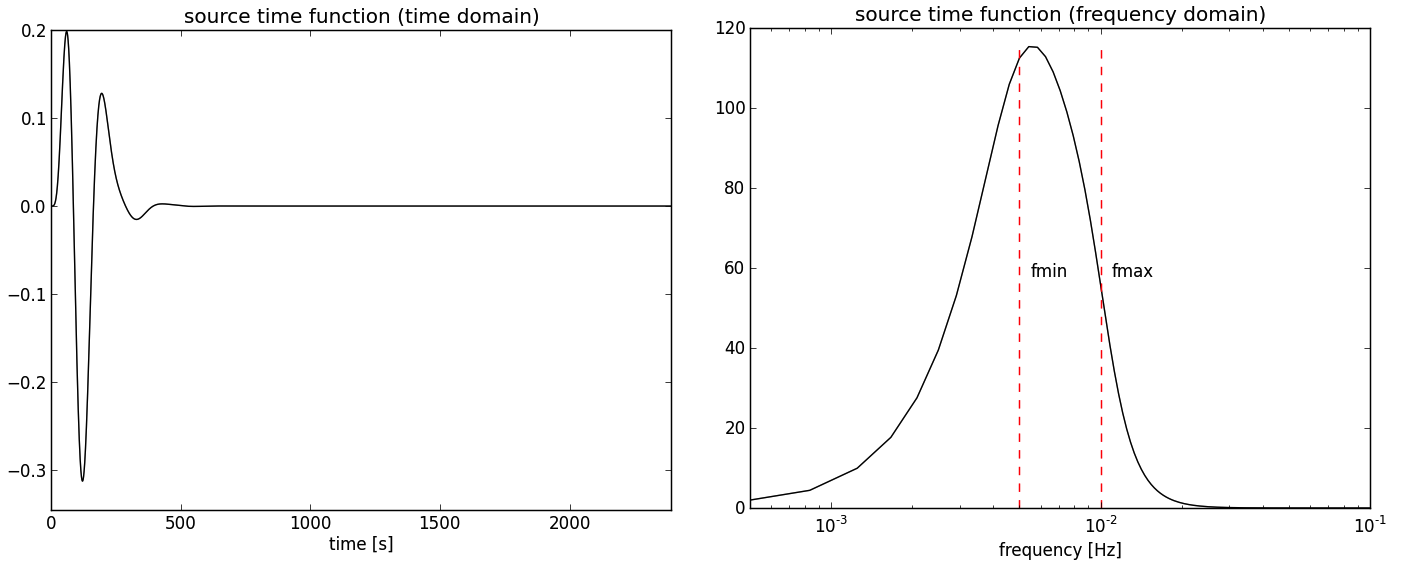
\includegraphics{Figures/stf_NA.png}} 
\caption{Time- and frequency-domain representation of the source time function produced by \texttt{make\_stf(0.2,12000,1.0/200.0,1.0/100.0,'../INPUT/stf')}}\label{F:stf_NA}
\end{figure}
\end{center}
%====================================================================

%====================================================================
% Constructing the 3D model.
%====================================================================

\subsection{Constructing the 3D model}

The construction of a 3D Earth model for this scenario is similar to the previous one described in section \ref{S:Anatolia}. The only difference is that the coordinates in the \texttt{block\_x}, \texttt{block\_y} and \texttt{block\_z} files must of course be rotated towards the equator.\\[5pt]
In the first step, we again generate a 1D model using \texttt{generate\_models}. As 1D model we choose one where all elastic parameters are set to zero, and where a smoothed version of the Q model QL6 (Durek \& Ekstr\"{o}m, 1996) is implemented. To use this model, set \texttt{model\_type} to \texttt{3} in the \texttt{setup} file. More details on visco-elastic dissipation for this specific scenario and from a more mathematical perspective can be found in sections \ref{S:NAQ} and \ref{S:attenuation}, respectively.\\[5pt] 
Following this initial step, we add 3D heterogeneities, again using \texttt{add\_perturbation}. To ensure that the heterogeneities are properly implemented, we can visualise the material parameters on the spectral-element grid using thy Python tool \texttt{ses3d\_fields.py} in the \texttt{TOOLS} directory (see also section \ref{S:Python}). The resulting plot is shown in figure \ref{F:fields}.  
%====================================================================
\begin{center}
\begin{figure}
\center\scalebox{0.3}{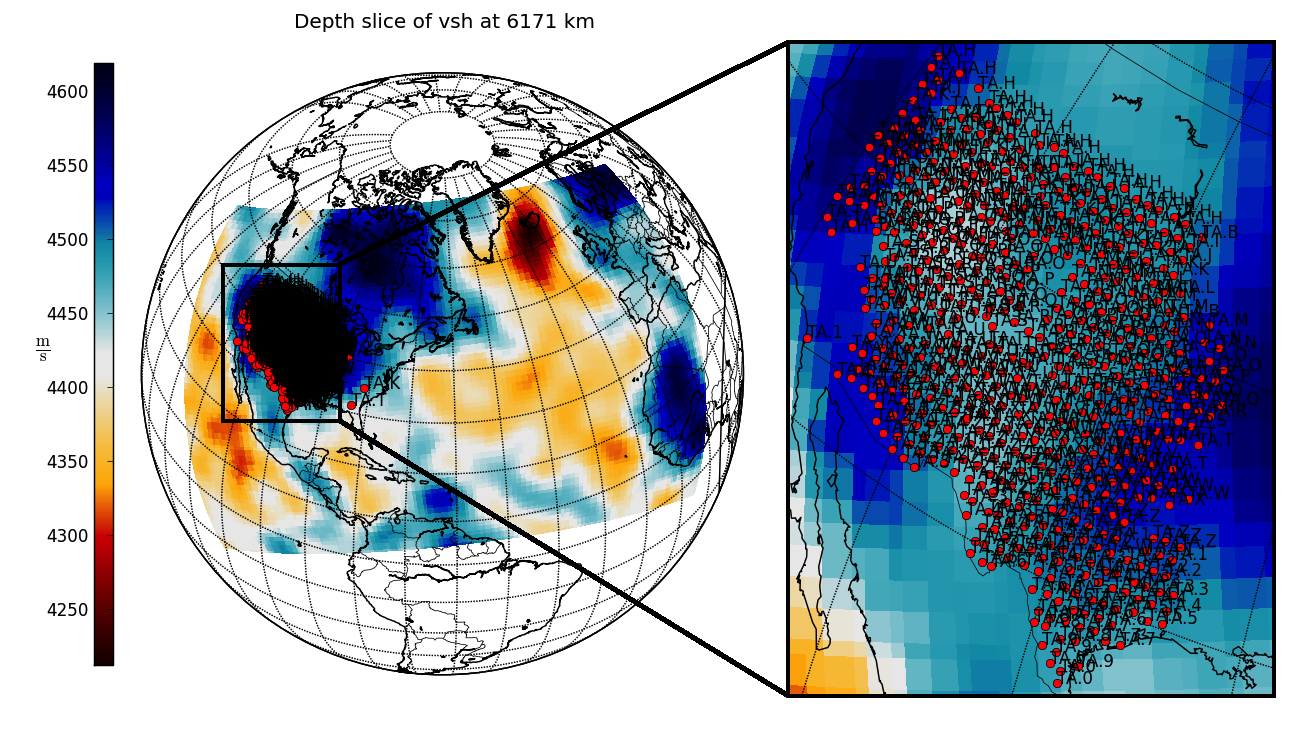
\includegraphics{Figures/fields.png}} 
\caption{Rotated North America model ($\vsv$) as implemented on the spectral-element grid. A zoom into the western part of USArray is shown to the right. This plot was made using \texttt{ses3d\_fields.py} from the \texttt{TOOLS} directory.}\label{F:fields}
\end{figure}
\end{center}
%====================================================================


\subsection{Visco-elastic dissipation}\label{S:NAQ}

To enable visco-elastic dissipation in \SES, the \texttt{is\_diss} flag in the \texttt{setup} file must be set to $1$. The mathematical description and numerical implementation of visco-elastic dissipation is described in chapter \ref{C:attenuation}. The visco-elastic properties of the Earth model are encoded in a set of relaxation parameters that can be computed using the Python code \texttt{Q\_discrete.py} located in the \texttt{TOOLS} directory. Requesting a constant $Q$ for periods between $80$ s and $250$ s, \texttt{Q\_discrete.py} produces the relaxation weights $1.684, 0.838, 1.357$, and the corresponding relaxation times $3.200, 17.692, 74.504$. These values must be written into the \texttt{relax} file in the \texttt{INPUT} directory. An illustration of the constant target $Q$ and the numerical approximation, as well as of the corresponding phase velocity dispersion, is provided in figure \ref{F:Q_NA}.
%====================================================================
\begin{center}
\begin{figure}
\center\scalebox{0.40}{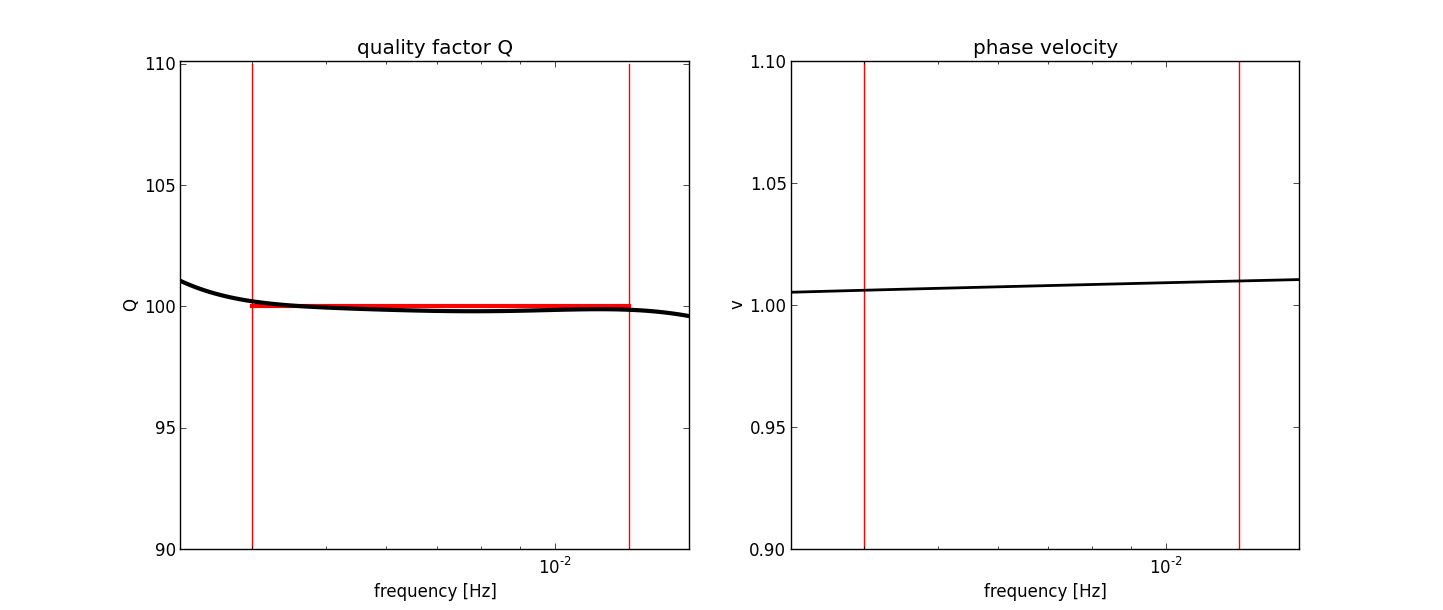
\includegraphics{Figures/Q_NA.png}} 
\caption{\textbf{Left}: Comparison of the constant target shear $Q$ with value $100$ and the corresponding numerical approximation, as computed by \texttt{Q\_discrete.py}. \textbf{Right}: Phase velocity dispersion.}\label{F:Q_NA}
\end{figure}
\end{center}
%====================================================================


\subsection{Wiggly lines}\label{S:NA_seismo}

To plot seismograms, we can use the Python class \texttt{ses3d\_seismogram} in the \texttt{TOOLS} directory. Simply run \texttt{seismograms.py} and then initiate a class member, e.g. by typing\\[5pt] 
\texttt{s=ses3d\_seismogram()}.\\[5pt] 
Using the \texttt{read} function, we can read a seismogram by giving the directory and station name:\\[5pt] \texttt{s.read('../DATA/OUTPUT/1/','TA.L16A\_.\_\_\_')}.\\[5pt]
Typing\\[5pt]
\texttt[s.plot()]\\[5pt]
will produce the plot shown in figure \ref{F:NA_seismo}. 
%====================================================================
\begin{center}
\begin{figure}
\center\scalebox{0.45}{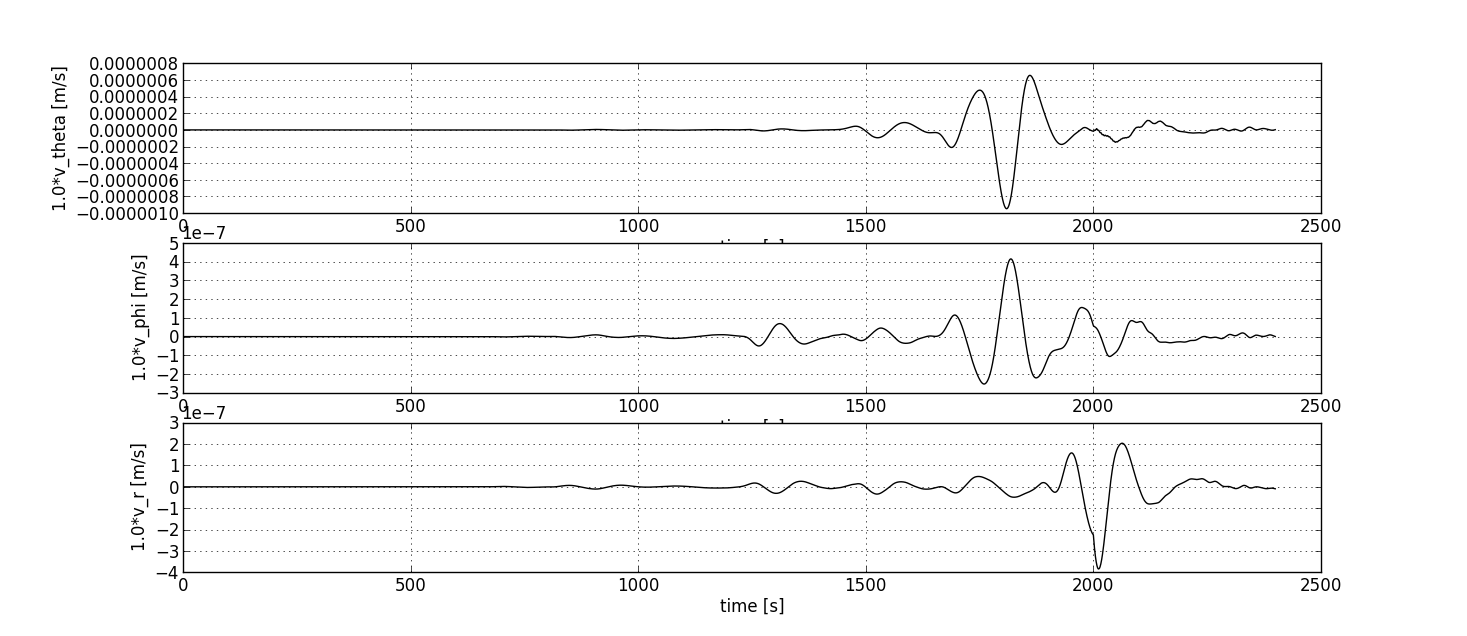
\includegraphics{Figures/seismo_example.png}} 
\caption{Three-component velocity seismograms at station TA.L16A.}\label{F:NA_seismo}
\end{figure}
\end{center}
%====================================================================
	\chapter{Python tools}\label{S:Python}

\SES comes with a collection of Python tools for visualisation, computing source time functions and adjoint sources, and various other purposes. All of these tools are located in the \texttt{TOOLS} directory. Being within \texttt{python} or \texttt{ipython}, a instructions for the use of these tools can be obtained by simply typing \texttt{help(name of the tool)}. Required Python packages include \href{www.numpy.org}{Numpy}, \href{www.scipy.org}{Scipy}, \href{http://matplotlib.org}{Matplotlib}, \href{http://matplotlib.org/basemap/}{Basemap} and \href{www.obspy.org}{Obspy}.The following is a commented list of currently available tools:

%%%%%%%%%%%%%%%%%%%%%%%%%%%%%%%%%%%%%%%%%%%%%%%%%%%%%%%%%%%%%%%%%%%
\section{Visualising and editing Earth models, snapshots and kernels}

\subsection{Visualising 3-D fields defined in terms of constant-property blocks}

Three-dimensional fields, including Earth models, velocity snapshots and sensitivity kernels, can be visualised with the help of \texttt{models.py}, provided that they are parametrised in the form described in section \ref{S:3Dmodels}. An instance of the class \texttt{ses3d\_model} can use the function \texttt{read} to read a 3-D field from a file given in terms of the path and filename. For this, the appropriate \texttt{block\_*} files must be in that path as well. A vertical slice can be plotted using the function \texttt{plot\_slice}. 

\subsection{Writing 3-D fields defined in terms of constant-property blocks}

After reading a 3-D field as described in the previous paragraph, the field may be manipulated and then written again using the \texttt{write} function of the \texttt{ses3d\_model} class.

\subsection{Converting 3-D fields defined in terms of constant-property blocks into vtk format}

For more elaborate visualisation, for instance in \href{www.paraview.org}{Paraview} or \href{https://wci.llnl.gov/codes/visit/}{VisIt}, the 3-D fields need to be converted into the vtk format. The function \texttt{convert\_to\_vtk} of the \texttt{ses3d\_model} class performs this conversion task.

\subsection{Visualising Earth models and velocity snapshots on the spectral-element grid}

The Python class \texttt{ses3d\_fields} contains tools for the visualisation of Earth models and velocity field snapshots defined on the spectral-element grid of SES3D. To plot, for instance, $\vsh$ at $20$ km depth with a colourbar ranging from $2698.0$ m$/$s to $3972.0$ m$/$s with a high-resolution coastline, just type\\[5pt]
\texttt{run ses3d\_fields.py\\
field=ses3d\_fields('../','/MODELS/MODELS/','earth\_model')\\
field.plot\_depth\_slice('vsh',20.0,2698.0,3872.0,res='h')}\\[5pt]
The first path '../' denotes the parent directory of the SES3D project, and the second '/MODELS/MODELS/' is the location of the Earth model parameters. Similarly, for plotting velocity field snapshots for $v_x$ at $100$ km depth and at iteration $1000$, type\\[5pt]
\texttt{run ses3d\_fields.py\\
field=ses3d\_fields('../','/DATA/OUTPUT/','velocity\_snapshot')\\
field.plot\_depth\_slice('vx',100.0,-9e-8,9e-8,iteration=1000,res='h')}\\


%%%%%%%%%%%%%%%%%%%%%%%%%%%%%%%%%%%%%%%%%%%%%%%%%%%%%%%%%%%%%%%%%%%
\section{Computing source time functions}

Source time functions can be computed and stored using \texttt{make\_stf.py}. Source time functions are computed as bandpass filtered Heaviside functions. \texttt{make\_stf.py} is deliberately simplistic. For real-data applications you must ensure that the bandpass applied in \texttt{make\_stf.py} is \emph{exactly} the bandpass applied to the data. Thus, you may want to adjust \texttt{make\_stf.py} to your specific needs. An example for the computation of a source time function can be found in section \ref{S:stf_NA}.


%%%%%%%%%%%%%%%%%%%%%%%%%%%%%%%%%%%%%%%%%%%%%%%%%%%%%%%%%%%%%%%%%%%
\section{Computing adjoint sources}

Code for the computation of adjoint sources for some simple measurements can be found in \texttt{adjoint\_source.py}. This tools fetches an \SES seismogram, makes a measurement in a pre-defined time window, and then computes the corresponding adjoint source. In the absence of real data, only data-independent adjoint sources can be computed. The currently implemented measurements are the cross-correlation traveltime shift, relative amplitude differences, multi-taper phase shifts and multi-taper amplitude differences. A concrete example for the computation of adjoint sources is given in section \ref{S:kernels}.


%%%%%%%%%%%%%%%%%%%%%%%%%%%%%%%%%%%%%%%%%%%%%%%%%%%%%%%%%%%%%%%%%%%
\section{Computing relaxation parameters of $Q$ models}

As described in chapter \ref{C:attenuation}, visco-elastic dissipation in \SES is described by a superposition of a finite number of relaxation mechanisms. The weights of these mechanisms and their respective relaxation times determine the behavior of $Q$ within a pre-defined frequency band. The Python code \texttt{Q\_discrete.py} computes these weights and relaxation times. The input parameters (frequency band, number of mechanisms, ...) must be given directly in the input section of the code, i.e. they are not passed as parameters to a function (because there are just too many parameters). A concrete example for the computation of relaxation weights and times can be found in section \ref{S:NAQ}.

%%%%%%%%%%%%%%%%%%%%%%%%%%%%%%%%%%%%%%%%%%%%%%%%%%%%%%%%%%%%%%%%%%%
\section{Rotating coordinates and moment tensors}

When working with a rotated coordinate system, a little set of tools for rotating coordinates and moment tensors is useful. These can be found in \texttt{rotation.py}. \texttt{rotate\_coordinates} rotates coordinates (colatitude and longitude) and \texttt{rotate\_moment\_tensor} rotates moment tensors. A detailed description is provided in the Python code itself.

%%%%%%%%%%%%%%%%%%%%%%%%%%%%%%%%%%%%%%%%%%%%%%%%%%%%%%%%%%%%%%%%%%%
\section{Reading and plotting seismograms}

The code \texttt{seismograms.py} contains the definition of the \texttt{ses3d\_seismogram} class that can be used to read and visualise synthetic seismograms produced by \SES. A detailed example can be found in section \ref{S:NA_seismo}.                            

%- inverse problem %%%%%%%%%%%%%%%%%%%%%%%%%%%%%%%%%%%%%%%%%%%%%%%%%%%%%%%%%%%

\begin{partbacktext}
\part{Mathematical background}


\end{partbacktext}
          

	\chapter{The seismic wave equation}\label{C:AnalyticalSetup}

This chapter is concerned with the mathematical description of
seismic wave propagation in the Earth and the derivation of
equations that can be solved numerically in an efficient way.
Following a brief review of the elastic wave equation and its
subsidiary conditions in section \ref{S:wave_equation}, we elaborate
on the simulation of anisotropy (section \ref{S:anisotropy}) and
attenuation (section \ref{S:attenuation}). We also cover the
implementation and analysis of absorbing boundaries within this
chapter on the analytical setup, because their properties are
relatively independent from a particular numerical scheme.

\section{The elastic wave equation}\label{S:wave_equation}

The propagation of seismic waves in the Earth can be modelled with
the elastic wave equation
\begin{equation}\label{E:into_waveeq001}
\rho(\w{x})\ddot{\w{u}}(\w{x}, t) - \nabla\cdot\s{\sigma}(\w{x}, t)
= \w{f}(\w{x}, t)\,,
\end{equation}
that relates the displacement field $\w{u}$ to the mass density
$\rho$, the stress tensor $\s{\sigma}$ and an external force density
$\w{f}$ (e.g. Dahlen \& Tromp, 1998; Kennett, 2001; Aki \& Richards, 2002). The elastic wave
equation as presented above is a linearised version of the momentum
balance equation, i.e., of Newton's second law. It is valid under
the assumption that deviations from the reference configuration of
the Earth are small. Furthermore, the rotation of the Earth and its
self-gravitation are omitted. These effects are negligible when
oscillation periods are shorter than $\sim 200$ s. At the surface
$\delta\oplus$ of the Earth $\oplus$ the normal components of the
stress tensor $\s{\sigma}$ vanish:
\begin{equation}\label{E:into_waveeq002}
\s{\sigma}\cdot\w{e}_r |_{\w{x}\in\partial\oplus} = \w{0}\,.
\end{equation}
Equation (\ref{E:into_waveeq002}) is the free surface boundary
condition. Both the displacement field $\w{u}$ and the velocity
field $\w{v}=\dot{\w{u}}$ are required to vanish prior to $t=t_0$
when the external force $\w{f}$ starts to act, i.e.,
\begin{equation}\label{E:into_waveeq003}
\w{u}|_{t<t_0}=\w{v}|_{t<t_0}=\w{0}\,.
\end{equation}
For convenience we will mostly choose $t_0=0$. To obtain a complete
set of equations, the stress tensor $\s{\sigma}$ has to be related
to the displacement field $\w{u}$. It is usually assumed that the
rheology is visco-elastic, meaning that the current stress tensor
$\s{\sigma}$ depends linearly on the history of the strain tensor
$\s{\epsilon}=\frac{1}{2}(\nabla \w{u} + \nabla \w{u}^T)$:
\begin{equation}\label{E:intro_waveeq004}
\s{\sigma}(\w{x}, t) = \int\limits_{-\infty}^{\infty}
\w{\dot{C}}(\w{x}, t-t'):\s{\epsilon}(\w{x}, t')\,dt'\,.
\end{equation}
The fourth order tensor $\w{C}$ is the elastic tensor. In the case
of a perfectly elastic medium the elastic tensor is of the form
$\w{C}(\w{x},t)=\w{C}(\w{x})\,H(t)$, where $H$ is the Heaviside
function. We then have $\s{\sigma}=\w{C}(\w{x}):\s{\epsilon}(\w{x},
t)$. The symmetry of $\s{\epsilon}$, the conservation of angular
momentum and the relation of $\w{C}$ to the internal energy (e.g.
Dahlen \& Tromp, 1998) require that the components of $\w{C}$
satisfy the following symmetry relations:
\begin{equation}\label{E:intro_waveeq005}
C_{ijkl}=C_{klij}=C_{jikl}\,.
\end{equation}
Moreover, the elastic tensor is causal:
\begin{equation}\label{E:into_waveeq006}
\w{C}(t)|_{t<t_0}=\w{0}\,.
\end{equation}
Equation (\ref{E:intro_waveeq004}) is $-$ unlike the wave equation
within its limits of validity $-$ not a fundamental law of physics
but an empirical relation that has been found to describe a wide
range of phenomena very well. It can be regarded as a linearisation
of a more general non-linear constitutive relation. Its validity is,
in this sense, restricted to scenarios where the strain tensor
$\s{\epsilon}$ is a small quantity. The particular choices of
$\w{C}$ and its time dependence will be the subjects of the
following sections on attenuation and anisotropy.

\section{Anisotropy}\label{S:anisotropy} 
Anisotropy is the dependence of the elastic tensor on the orientation of the
coordinate system. Its most direct seismological expression is the
dependence of seismic velocities on the propagation and polarisation
directions of elastic waves. It is thought to play a major role in the Earth's crust and upper mantle.\\
Besides the splitting of shear waves, the Love wave-Rayleigh wave
discrepancy is one of the principal seismic observations that is
directly related to anisotropy: A Love wave and a Rayleigh wave
travelling in the same direction usually exhibit different wave
speeds as a consequence of their different polarisations. This led
to the inclusion of anisotropy with radial symmetry axis in the
global reference model PREM (Dziewonski \& Anderson, 1981). In this
model the anisotropy
is limited to the upper 220 km.\\
Guided by these observations, we decided to implement anisotropy
with radial symmetry axis. For such a medium, there are only 5
independent elastic tensor components that are different from zero.
They can be summarised in a $6\times 6$ matrix (e.g. Babuska \& Cara, 1991):
\begin{align}\label{E:setup15}
&\begin{pmatrix}
C_{r r r r} & C_{r r \phi \phi} & C_{r r \theta \theta} & C_{r r \phi \theta} & C_{r r r \theta} & C_{r r r \phi} \\
C_{\phi \phi r r} & C_{\phi \phi \phi \phi} & C_{\phi \phi \theta \theta} & C_{\phi \phi \phi \theta} & C_{\phi \phi r \theta} & C_{\phi \phi r \phi} \\
C_{\theta \theta r r} & C_{\theta \theta \phi \phi} & C_{\theta \theta \theta \theta} & C_{\theta \theta \phi \theta} & C_{\theta \theta r \theta} & C_{\theta \theta r \phi} \\
C_{\phi \theta r r} & C_{\phi \theta \phi \phi} & C_{\phi \theta \theta \theta} & C_{\phi \theta \phi \theta} & C_{\phi \theta r \theta} & C_{\phi \theta r \phi} \\
C_{r \theta r r} & C_{r \theta \phi \phi} & C_{r \theta \theta \theta} & C_{r \theta \phi \theta} & C_{r \theta r \theta} & C_{r \theta r \phi} \\
C_{r \phi r r} & C_{r \phi \phi \phi} & C_{r \phi \theta \theta} &
C_{r \phi \phi \theta} & C_{r \phi r \theta} & C_{r \phi r \phi}
\end{pmatrix}\notag\\
=&
\begin{pmatrix}
\lambda+2\mu & \lambda+c & \lambda+c & 0 & 0 & 0 \\
\lambda+c & \lambda+2\mu+a & \lambda+a & 0 & 0 & 0 \\
\lambda+c & \lambda+a & \lambda+2\mu+a & 0 & 0 & 0 \\
0 & 0 & 0 & \mu & 0 & 0 \\
0 & 0 & 0 & 0 & \mu+b & 0 \\
0 & 0 & 0 & 0 & 0 & \mu+b
\end{pmatrix}
\end{align}
Love (1892) proposed an alternative parametrisation
\begin{align}\label{E:setup15b}
&\begin{pmatrix}
C_{r r r r} & C_{r r \phi \phi} & C_{r r \theta \theta} & C_{r r \phi \theta} & C_{r r r \theta} & C_{r r r \phi} \\
C_{\phi \phi r r} & C_{\phi \phi \phi \phi} & C_{\phi \phi \theta \theta} & C_{\phi \phi \phi \theta} & C_{\phi \phi r \theta} & C_{\phi \phi r \phi} \\
C_{\theta \theta r r} & C_{\theta \theta \phi \phi} & C_{\theta \theta \theta \theta} & C_{\theta \theta \phi \theta} & C_{\theta \theta r \theta} & C_{\theta \theta r \phi} \\
C_{\phi \theta r r} & C_{\phi \theta \phi \phi} & C_{\phi \theta \theta \theta} & C_{\phi \theta \phi \theta} & C_{\phi \theta r \theta} & C_{\phi \theta r \phi} \\
C_{r \theta r r} & C_{r \theta \phi \phi} & C_{r \theta \theta \theta} & C_{r \theta \phi \theta} & C_{r \theta r \theta} & C_{r \theta r \phi} \\
C_{r \phi r r} & C_{r \phi \phi \phi} & C_{r \phi \theta \theta} &
C_{r \phi \phi \theta} & C_{r \phi r \theta} & C_{r \phi r \phi}
\end{pmatrix}\notag\\
=&
\begin{pmatrix}
C_L & F_L & F_L & 0 & 0 & 0 \\
F_L & A_L & A_L-2N_L & 0 & 0 & 0 \\
F_L & A_L-2N_L & A_L & 0 & 0 & 0 \\
0 & 0 & 0 & N_L & 0 & 0 \\
0 & 0 & 0 & 0 & L_L & 0 \\
0 & 0 & 0 & 0 & 0 & L_L
\end{pmatrix}
\end{align}
We chose to use the parametrisation from equation (\ref{E:setup15})
because it easily allows us to model isotropy by simply setting
$a=b=c=0$. Remember, that all components of the elastic tensor are
functions of time, $t$, and space, $\w{x}$. Density, $\rho$ and the
elastic parameters $\lambda, \mu, a, b$ and $c$ can be related to
the wave speeds of SH, SV, PH and PV waves:
\begin{equation}\label{E:svsh17}
\vsv=\sqrt{\frac{\mu+b}{\rho}}\,,\quad
\vsh=\sqrt{\frac{\mu}{\rho}}\,,\quad
\vpv=\sqrt{\frac{\lambda+2\mu}{\rho}}\,,\quad
\vph=\sqrt{\frac{\lambda+2\mu+a}{\rho}}\,.
\end{equation}
The velocities of SH, SV, PH and PV waves specify only two of the
three additional elastic parameters necessary for anisotropy with
radial symmetry axis, namely $a$ and $b$. Also radially propagating
S waves do not allow us to find $c$, because they propagate with the
velocity $\sqrt{(\mu+b)/\rho}$, just as SV waves. In fact, using
plane waves, $c$ can be determined only from P waves that do not
travel in exactly radial or horizontal directions. Following
Takeuchi \& Saito (1972) and Dziewonski \& Anderson (1981) we
incorporate $c$ into a dimensionless parameter
\begin{equation}\label{E:pvph007}
\eta:=(\lambda+c)/(\lambda+a)\,.
\end{equation}
        
	\chapter{Description and implementation of attenuation}\label{C:attenuation}

%%%%%%%%%%%%%%%%%%%%%%%%%%%%%%%%%%%%%%%%%%%%%
% The visco-elastic rheology and memory variables
%%%%%%%%%%%%%%%%%%%%%%%%%%%%%%%%%%%%%%%%%%%%%

\section{The visco-elastic rheology and memory variables}\label{S:attenuation}

The numerical implementation of attenuation is largely motivated by
technical convenience and not so much by the true physics of seismic
wave attenuation in the interior of the Earth. In our analysis we closely follows Robertsson et al. (1994),
but introduce some modifications that facilitate the construction of constant-$Q$ models.\\
Assume that $\sigma, C$ and $\epsilon$ are representative of some
particular components of $\s{\sigma}, \w{C}$ and $\s{\epsilon}$,
respectively. Then a scalar version of the stress-strain relation is
given by
\begin{equation}\label{E:setup16}
\dot{\sigma}(t) = (\dot{C}*\dot{\epsilon})(t) =
\int\limits_{-\infty}^{\infty} \dot{C}(t-t') \dot{\epsilon}(t')\,
dt'\,.
\end{equation}
The spatial dependence has been omitted for brevity. As already
discussed, we choose the stress relaxation function or elastic
tensor component $C$ to be that of a superposition of $N$ standard
linear solids, weighted by coefficients $D_p$ ($p=1, ..., N)$, i.e.,
\begin{equation}\label{E:setup17}
C(t) := C_r \left[ 1- \sum_{p=1}^{N} D_p\, \left( 1-
\frac{\tau_{\epsilon p}}{\tau_{\sigma p}}\right)\,e^{-t/\tau_{\sigma
p}}\right] \, H(t)\,,
\end{equation}
where $\tau_{\epsilon p}$ and $\tau_{\sigma p}$ are the strain and
stress relaxation times of the $p$th standard linear solid,
respectively. The symbol $H$ denotes the Heaviside function and
$C_r$ is the relaxed modulus. Equation (\ref{E:setup17}) is very
general so that  different sets of relaxation times can give almost
the same relaxation function $C(t)$. To reduce this subjectively
undesirable non-uniqueness we limit the number of free parameters.
Following the $\tau$-method introduced by Blanch et al. (1995) we
determine the relaxation times $\tau_{\epsilon p}$ by defining a
dimensionless variable $\tau$ through
\begin{equation}\label{E:setup18}
\tau := \frac{\tau_{\epsilon p}}{\tau_{\sigma p}} -1\, .
\end{equation}
This gives
\begin{equation}\label{E:setup19}
C(t) = C_r \left[ 1+\tau\, \sum_{p=1}^{N} D_p\, e^{-t/\tau_{\sigma
p}} \right]\, H(t)\,.
\end{equation}
Differentiating (\ref{E:setup19}) with respect to $t$ and
introducing the result into equation (\ref{E:setup16}) yields
\begin{equation}\label{E:setup20}
\dot{\sigma}(t) = C_r (1+s\,\tau)\,\dot{\epsilon}(t) + C_r
\sum_{p=1}^{N} M_p\,,\quad s:=\sum_{p=1}^N D_p
\end{equation}
where the memory variables $M_p$ are defined by
\begin{equation}\label{E:setup21}
M_p := -\frac{D_p\,\tau}{\tau_{\sigma
p}}\,\int\limits_{-\infty}^{\infty} e^{-(t-t')/\tau_{\sigma p}}\,
H(t-t')\,\dot{\epsilon}(t')\, dt'\,.
\end{equation}
The differentiation of (\ref{E:setup21}) with respect to time yields
a set of first-order differential equations for the memory
variables:
\begin{equation}\label{E:setup22}
\dot{M_p} = -\frac{D_p\,\tau}{\tau_{\sigma p}} \, \dot{\epsilon} -
\frac{1}{\tau_{\sigma p}}\, M_p\,.
\end{equation}
Anelasticity can thus be modelled by simultaneously sloving the
momentum equation, a modified stress-strain relation and a set of
$N$ ordinary differential equations for the memory variables $M_p$.
The memory variables are formally independent of the elastic
parameter $C_r$. This formulation, proposed by Moczo \& Kristek
(2005), gives more accurate results in the case of strong attenuation heterogeneities than the classical formulation by Robertsson et al. (1994).\\
Generalising equations (\ref{E:setup20}) and (\ref{E:setup22}) to
the case of a three-dimensional and anisotropic medium with radial
symmetry axis is straightforward. The component-wise stress-strain
relation in the absence of dissipation is given by the following set
of equations:
\begin{subequations}\label{E:setup32}
\begin{align}
\sigma_{rr}&=(\kappa-2\mu/3)(\epsilon_{rr}+\epsilon_{\theta\theta}+\epsilon_{\phi\phi})+2\mu\epsilon_{rr}+c(\epsilon_{\theta\theta}+\epsilon_{\phi\phi})\\
\sigma_{\phi\phi}&=(\kappa-2\mu/3)(\epsilon_{rr}+\epsilon_{\theta\theta}+\epsilon_{\phi\phi})+2\mu\epsilon_{\phi\phi}+c\epsilon_{rr}+a(\epsilon_{\theta\theta}+\epsilon_{\phi\phi})\\
\sigma_{\theta\theta}&=(\kappa-2\mu/3)(\epsilon_{rr}+\epsilon_{\theta\theta}+\epsilon_{\phi\phi})+2\mu\epsilon_{\theta\theta}+c\epsilon_{rr}+a(\epsilon_{\theta\theta}+\epsilon_{\phi\phi})\\
\sigma_{r\phi}&=2(\mu+b)\epsilon_{r\phi}\\
\sigma_{r\theta}&=2(\mu+b)\epsilon_{r\theta}\\
\sigma_{\phi\theta}&=2\mu\epsilon_{\phi\theta}
\end{align}
\end{subequations}
We introduced the bulk modulus $\kappa=\lambda+\frac{2}{3}\mu$
because it is $-$ in contrast to the Lam\'{e} parameter $\lambda$ $-$
physically interpretable.\footnote{\textsf{There is, to the best of
my knowledge, no physical interpretation of $\lambda$. The
unphysical nature of this parameter becomes most apparent through
the fact that the $Q$ factor associated with $\lambda$, denoted by
$Q_\lambda$, can be negative for positive $Q_\mu$ and $Q_\kappa$.
Thus, if there were a physical process, e.g. an elastic wave, that
depended only on $\lambda$ and $\rho$, then this process would go
hand in hand with a continuously growing elastic energy.}} The
transition to the dissipative medium is now made by analogy:
\begin{subequations}\label{E:setup33}
\begin{align}
\dot{\sigma}_{rr}&=\left[\kappa_r
(1+s_\kappa \tau_\kappa)-\frac{2}{3}\mu_r(1+s_\mu \tau_\mu)\right]\,(\dot{\epsilon}_{rr}+\dot{\epsilon}_{\theta\theta}+\dot{\epsilon}_{\phi\phi})+2\mu_r(1+s_\mu\,\tau_\mu)\dot{\epsilon}_{rr}+c(\dot{\epsilon}_{\theta\theta}+\dot{\epsilon}_{\phi\phi})\notag\\
&+\kappa_r\sum_{p=1}^N \left(
K_{p}^{rr}+K_{p}^{\theta\theta}+K_{p}^{\phi\phi}\right)
-\frac{2}{3}\mu_r \sum_{p=1}^{N} \left(
M_p^{\theta\theta}+M_p^{\phi\phi} \right) + \frac{4}{3} \mu_r
\sum_{p=1}^{N} M_p^{rr}\\
\dot{\sigma}_{\phi\phi}&=\left[\kappa_r
(1+s_\kappa \tau_\kappa)-\frac{2}{3}\mu_r(1+s_\mu \tau_\mu)\right]\,(\dot{\epsilon}_{rr}+\dot{\epsilon}_{\theta\theta}+\dot{\epsilon}_{\phi\phi})+2\mu_r(1+s_\mu \tau_\mu)\dot{\epsilon}_{\phi\phi}+c\dot{\epsilon}_{rr}+a(\dot{\epsilon}_{\theta\theta}+\dot{\epsilon}_{\phi\phi})\notag\\
&+\kappa_r\sum_{p=1}^N \left(
K_{p}^{rr}+K_{p}^{\theta\theta}+K_{p}^{\phi\phi}\right)-\frac{2}{3}\mu_r
\sum_{p=1}^{N}
\left(M_p^{rr}+M_p^{\theta\theta}\right)+\frac{4}{3}\mu_r
\sum_{p=1}^{N} M_p^{\phi\phi}\\
\dot{\sigma}_{\theta\theta}&=\left[\kappa_r
(1+s_\kappa \tau_\kappa)-\frac{2}{3}\mu_r(1+s_\mu \tau_\mu)\right]\,(\dot{\epsilon}_{rr}+\dot{\epsilon}_{\theta\theta}+\dot{\epsilon}_{\phi\phi})+2\mu_r(1+s_\mu \tau_\mu)\dot{\epsilon}_{\theta\theta}+c\dot{\epsilon}_{rr}+a(\dot{\epsilon}_{\theta\theta}+\dot{\epsilon}_{\phi\phi})\notag\\
&+\kappa_r\sum_{p=1}^N \left(
K_{p}^{rr}+K_{p}^{\theta\theta}+K_{p}^{\phi\phi}\right)-\frac{2}{3}\mu_r
\sum_{p=1}^{N} \left(M_p^{rr}+M_p^{\phi\phi}\right)+\frac{4}{3}\mu_r
\sum_{p=1}^{N} M_p^{\theta\theta}\\
\dot{\sigma}_{r\phi}&=2\mu_r(1+s_\mu \tau_\mu)\dot{\epsilon}_{r\phi}+2b\dot{\epsilon}_{r\phi}+2\mu_r\sum_{p=1}^{N}
M_p^{r\phi}\\
\dot{\sigma}_{r\theta}&=2\mu_r(1+s_\mu \tau_\mu)\dot{\epsilon}_{r\theta}+2b\dot{\epsilon}_{r\phi}+2\mu_r\sum_{p=1}^{N}
M_p^{r\theta}\\
\dot{\sigma}_{\phi\theta}&=2\mu_r(1+s_\mu \tau_\mu)\dot{\epsilon}_{\phi\theta}+2\mu_r
\sum_{p=1}^{N} M_p^{\phi\theta}
\end{align}
\end{subequations}
For equations (\ref{E:setup33}) we assumed that the parameters $a,
b$ and $c$ are not involved in the dissipation of elastic energy.
The memory variables associated with $\mu$ $-$ denoted by $M_p^{ij}$
$-$ and the memory variables associated with $\kappa$ $-$ denoted by
$K_p^{ij}$ $-$ are governed by the first-order differential
equations
\begin{align}\label{E:setup34}
\dot{M}_p^{ij}&=-\frac{D_{p,\mu}\,\tau_\mu}{\tau_{\sigma p, \mu}}
\dot{\epsilon}_{ij} - \frac{1}{\tau_{\sigma p,\mu}} M_{p}^{ij}\\
\dot{K}_p^{ij}&=-\frac{D_{p,\kappa}\,\tau_\kappa}{\tau_{\sigma p, \kappa}}
\dot{\epsilon}_{ij} - \frac{1}{\tau_{\sigma p,\kappa}} K_{p}^{ij}
\end{align}
The above description of anelasticity is computationally inexpensive
compared to the spatial discretisation of the equations of motion
which account for the largest portion of the computational costs.

%%%%%%%%%%%%%%%%%%%%%%%%%%%%%%%%%%%%%%%%%%%%%
% Q and velocity dispersion
%%%%%%%%%%%%%%%%%%%%%%%%%%%%%%%%%%%%%%%%%%%%%

\section{$Q$ and phase velocity dispersion}

In seismology there has traditionally been more emphasis on the
quality factor Q than on particular stress or strain relaxation
functions. The definition of $Q$ is based on the definition of the
complex modulus
\begin{equation}\label{E:setup28}
\mathcal{C}(\nu) := \w{i}\,\nu\,\int_{0}^{\infty} C(t)\,e^{-\w{i}\nu
t}\, dt\,,
\end{equation}
with $\nu:=\omega+\w{i}\gamma$ and the damping factor $\gamma<0$. Then
\begin{equation}\label{E:setup29}
Q(\omega) :=
\frac{\frak{Re}\,\mathcal{C}(\omega)}{\frak{Im}\,\mathcal{C}(\omega)}\,.
\end{equation}
For our stress relaxation function defined in equation
(\ref{E:setup19}) we find
\begin{equation}\label{E:setup31a}
\mathcal{C}(\omega)=C_r + \w{i}\omega C_r\,\tau\,\sum_{p=1}^{N} \frac{D_p}{\w{i}\omega + \tau_{\sigma p}^{-1}}=A(\omega)+\w{i}\,B(\omega)\,,
\end{equation}
with the real and imaginary parts
\begin{equation}\label{E:setup31c}
A(\omega)=C_r\,\left[1+\tau\,\sum_{p=1}^{N} \frac{D_p\omega^2 \tau_{\sigma p}^2}{1+\omega^2 \tau_{\sigma p}^2}\right]\,,\quad B(\omega)=C_r\tau\,\sum_{p=1}^{N} \frac{D_p \omega \tau_{\sigma p}}{1+\omega^2 \tau_{\sigma p}^2}\,.
\end{equation}
Therefore, $Q$ is explicitly given by
\begin{equation}\label{E:setup31b}
Q(\omega) = \frac{ \left( 1+ \sum_{p=1}^{N} \frac{D_p\,\omega^2
\tau_{\sigma p}^2\tau}{1+\omega^2 \tau_{\sigma p}^2} \right)}{
\sum_{p=1}^{N} \left( \frac{D_p\,\omega \tau_{\sigma p}
\tau}{1+\omega^2\tau_{\sigma p}^2} \right)}\,.
\end{equation}
Visco-elastic dissipation implies phase velocity dispersion, where the phase velocity $v$ is defined by
\begin{equation}\label{E:setup32}
v=\frac{\omega}{\frak{Re}\,k}\,.
\end{equation}
The wave number is determined by the dispersion relation
\begin{equation}\label{E:setup33}
k^2=\frac{\omega^2 \rho}{\mathcal{C}}\,,
\end{equation}
which follows directly from the one-dimensional wave equation with a spatially invariable $C$. After some algebra, we find
\begin{equation}\label{E:setup34}
(\frak{Re}\,k)^2=\frac{1}{2}\,\rho\omega^2\,\frac{A+\sqrt{A^2+B^2}}{A^2+B^2}\,,
\end{equation}
and
\begin{equation}\label{E:setup35}
v^2=\frac{2\,(A^2+B^2)}{\rho\,(A+\sqrt{A^2+B^2})}\,.
\end{equation}

%%%%%%%%%%%%%%%%%%%%%%%%%%%%%%%%%%%%%%%%%%%%%
% Q and the loss of elastic energy
%%%%%%%%%%%%%%%%%%%%%%%%%%%%%%%%%%%%%%%%%%%%%

\section{$Q$ and the loss of elastic energy}

The quality factor $Q$ and its most common interpretation is closely related to the loss of elastic energy, that finds its most prominent expression in the reduction of the displacement amplitude, as the wave progresses in time and space. To see this, we first write the solution of the scalar wave equation in terms of the real and imaginary parts of the complex wave number $k=k_r+\w{i}\,k_i$:
\begin{equation}\label{E:Qintro027}
u(x,t)=u_0 e^{\w{i}\,(k_r x-\omega t)}\,e^{-k_i x}\,.
\end{equation}
Equation (\ref{E:Qintro027}) reveals that $k_i$ describes the amplitde reduction with increasing propagation distance. Let us now determine $k_i$ explicitly, first in terms of $A$ and $B$. For $k_i$ we find
\begin{equation}\label{E:Qintro028}
k_i^2=\frac{1}{2} \frac{\rho\omega^2}{A^2+B^2}\left( \sqrt{A^2+B^2}-A \right)\,.
\end{equation}
Working under the assumption that $Q$ is large, i.e. $B$ is small, we find the first-order expression
\begin{equation}\label{E:Qintro029}
k_i^2 \approx \frac{1}{4} \frac{\rho\omega^2 A Q^{-1}}{A^2+B^2}\,.
\end{equation}
Furthermore, for large $Q$, we have $v^2\approx A/\rho$, and equation (\ref{E:Qintro029}) simplifies to
\begin{equation}\label{E:Qintro030}
k_i = \frac{\omega}{2vQ}\,,
\end{equation}
where we replaced $\approx$ by $=$ for clarity in the following expressions. Based on equation (\ref{E:Qintro030}) we find that the amplitude reduction is proportional to $\exp\left(-\frac{\omega x}{2vQ}\right)$, and that the elastic energy reduction is proportional to  $\exp\left(-\frac{\omega x}{vQ}\right)$. Thus, by progressing from position $x$ to position $x+\lambda$, where $\lambda$ is the wavelength, the fractional energy loss is, correct to first order, given by
\begin{equation}\label{E:Qintro031}
\frac{E(x+\lambda)-E(x)}{E(x)}=-\frac{2\pi}{Q}\,.
\end{equation}
Equation (\ref{E:Qintro031}) can be interpreted as the definition of the \emph{spatial $Q$}. Alternatively, we may substitute $x=vt$, and then ask how the energy is reduced during one temporal osciallation cycle, i.e., as we progress from time $t$ to time $t+T$, where $T=\lambda v^{-1}$ is the period. Then we find, again correct to first order,
\begin{equation}\label{E:Qintro032}
\frac{E(t+T)-E(t)}{E(t)}=-\frac{2\pi}{Q}\,.
\end{equation}
This defines the \emph{temporal $Q$}.

%%%%%%%%%%%%%%%%%%%%%%%%%%%%%%%%%%%%%%%%%%%%%
% Q models
%%%%%%%%%%%%%%%%%%%%%%%%%%%%%%%%%%%%%%%%%%%%%

\section{Constructing constant-$Q$ models}

\subsection{Continuous case}

We are interested in constructing $Q$ models that are approximately independent of frequency for circular frequencies $\omega$ that are within the absorption band
\begin{equation}\label{E:Qconst001}
\tau_1 \ll \omega^{-1} \ll \tau_2\,,
\end{equation}
where $\tau_1$ and $\tau_2$ are stress-relaxation times that define the boundaries of the absorption band. Constructing such constant-$Q$ models means to find a set of stress-relaxation times $\tau_{\sigma p}$ and weights $D_p$ such that $Q(\omega)\approx \text{const}$ for $\omega$ satisfying (\ref{E:Qconst001}). This is a difficult undertaking, which requires a non-linear optimisation of equation (\ref{E:setup17}).\\
To facilitate our analysis, we make a detour via the case of a continuous distribution of standard-linear solids, i.e. we generalise equation (\ref{E:setup17}) to
\begin{equation}\label{E:Qconst002}
C(t)=C_r\,\left[1+\tau\,\int_{0}^{\infty} D(\tau_\sigma)\,e^{-t/\tau_\sigma}\,d\tau_\sigma \right]\,H(t)\,.
\end{equation}
The complex modulus is then
\begin{equation}\label{E:Qconst004}
\mathcal{C}(\omega)=A(\omega)+\w{i}B(\omega)\,,
\end{equation}
with
\begin{equation}\label{E:Qconst005}
A(\omega)=C_r\,\left[1+\tau\,\int_0^\infty \frac{\omega^2 \tau_\sigma^2}{1+\omega^2\tau_\sigma^2}\,D(\tau_\sigma)\,d\tau_\sigma \right]\,,\quad B(\omega)=C_r\,\left[\tau\,\int_0^\infty \frac{\omega\tau_\sigma}{1+\omega^2\tau_\sigma^2} D(\tau_\sigma)\,d\tau_\sigma   \right]\,.
\end{equation}
Choosing
\begin{equation}\label{E:Qconst006}
D(\tau_\sigma)=\begin{cases}
&\tau_\sigma^{-1}\,,\quad \text{for}\quad \tau_1\leq\tau_\sigma\leq\tau_2\notag\\
& 0\,,\quad \text{otherwise} \end{cases}\,,
\end{equation}
we obtain
\begin{align}\label{E:Qconst007}
A(\omega)&=C_r\,\left[1+\frac{1}{2}\tau\,\ln\left(\frac{1+\omega^2\tau_2^2}{1+\omega^2 \tau_1^2}  \right)\right]\,,\\
B(\omega)&=C_r\tau\,\left[\arctan(\omega\tau_2)-\arctan(\omega\tau_1) \right]\,.
\end{align}
For $\omega$ well within the absorption band, we obtain the useful approximations
\begin{equation}\label{E:Qconst008}
Q^{-1}\approx\frac{1}{2}\,\tau\pi = \text{const.}\,,
\end{equation}
and
\begin{equation}\label{E:Qconst009}
v\approx \sqrt{\frac{C_r}{\rho}} \left[1+\frac{1}{\pi Q}\,\ln(\omega\tau_2)\right]\,.
\end{equation}
As desired, $Q$ is approximately constant. Furthermore, the phase velocity increases with increasing frequency. This result implies that the weights of the relaxation mechanisms in the discrete case, $D_p$, should be proportional to $\tau_{\sigma p}^{-1}$. The parameter $\tau$ controls the numerical value of $Q$, and the relaxation times $\tau_{\sigma p}$ control the width of the absorption band. An example is shown in figure \ref{F:absorption_continuous}.
%====================================================================
\begin{center}
\begin{figure}
\center\scalebox{0.45}{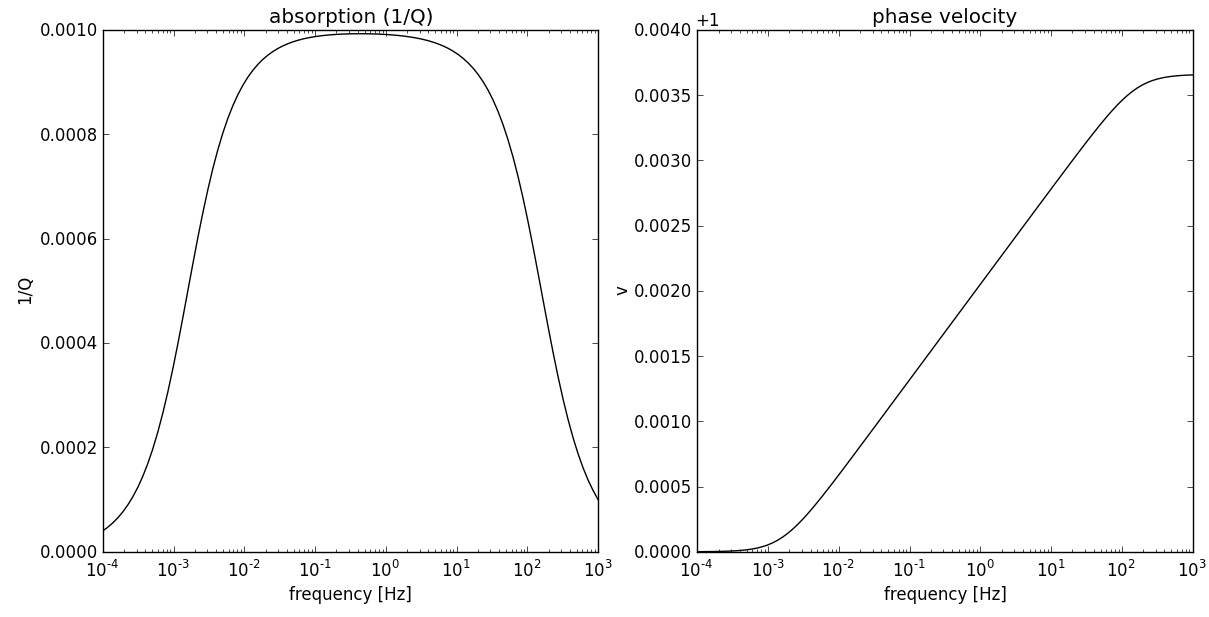
\includegraphics{Figures/absorption_band_continuous.jpg}} 
\caption{Example of a continuous absorption-band model with $Q=1000$, $\tau_1=1\cdot 10^{-3}$ s and $\tau_2=1\cdot 10^{2}$ s. The frequency-dependence of $Q^{-1}$ and the phase velocity $v$ are shown. This plot was produced using the Python tool \texttt{Q\_continuous.py} in the \texttt{TOOLS} directory.}\label{F:absorption_continuous}
\end{figure}
\end{center}
%====================================================================

\subsection{Discrete case}\label{S:Qdiscrete}

In the case of a discrete superposition of a finite number of relaxation mechanisms, the previous analysis is not sufficiently accurate because the frequency range considered is usually rather narrow. Therefore, we only take a few relaxation mechanisms (typically $2$ to $4$) with relaxation times $\tau_{\sigma p}$ and assign initial weights as $D_p=\tau_{\sigma p}$. Using a non-linear optimisation we then find optimal $\tau_{\sigma p}$ and $D_p$ such that
\begin{equation}\label{E:Qconst010}
\sum_{p=1}^{N} \frac{D_p \omega \tau_{\sigma p}}{1+\omega^2 \tau_{\sigma p}^2}=\frac{\pi}{2}\,,
\end{equation}
within the desired frequency band. For large $Q$, the relation between $Q$ and $\tau$ is then the same as for the continuous case:
\begin{equation}\label{E:Qconst011}
Q^{-1}\approx\frac{1}{2}\,\tau\pi \,.
\end{equation}
Figure \ref{F:absorption_discrete} shows an example.
%====================================================================
\begin{center}
\begin{figure}
\center\scalebox{0.45}{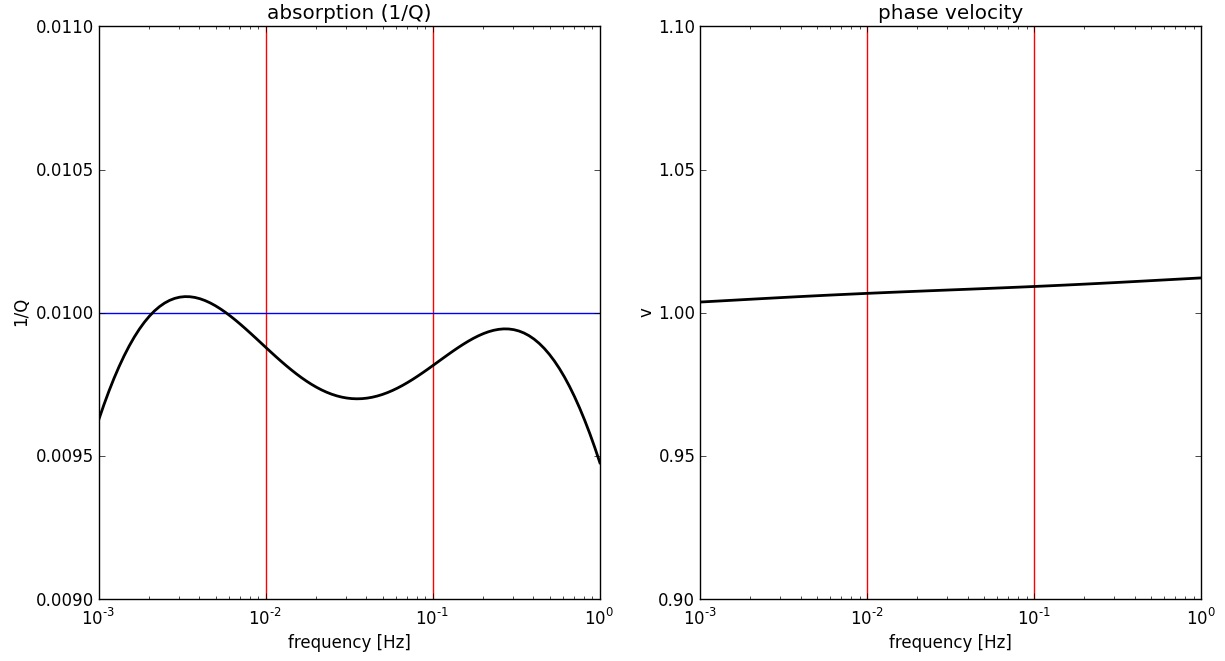
\includegraphics{Figures/absorption_band_discrete.jpg}} 
\caption{Example of a discrete absorption-band model with a constant target $Q=100$ in the frequency range $1\cdot 10^{-3}$-$1\cdot 10^{-2}$ Hz, which is indicated by red vertical lines. The number of relaxation mechanisms is $N=3$. This plot was produced using the Python tool \texttt{Q\_discrete.py} in the \texttt{TOOLS} directory.}\label{F:absorption_discrete}
\end{figure}
\end{center}
%====================================================================
	
\chapter{Absorbing boundaries}\label{S:absbound_theo}

Restricting the considered spatial domain to only a part of the true physical
domain in the interest of computational efficiency, introduces
unrealistic boundaries. If not treated adequately, the reflections
from the artificial boundaries dominate the numerical error. The
most widely used solutions for this problem fall into two
categories: \emph{absorbing boundary conditions} and \emph{absorbing
boundary layers}.\\
Absorbing boundary conditions are usually based on paraxial
approximations of the wave equation. Early applications of this
technique to finite-difference modelling can be found in Clayton \&
Engquist (1977) or in Stacey (1988). Along the artificial boundary the wave
equation is replaced by one of its paraxial approximations of order
$n$, typically not higher than one or two. The reflection
coefficient then behaves as $(\sin \phi)^n$, where $\phi$ is the
angle of incidence. Absorbing boundary conditions therefore become
inefficient for large angles of incidence in general and for surface
waves in particular. Moreover, they suffer from numerical stability
problems.\\
Absorbing boundary layers are regions near the unphysical boundaries
where the wave field is artificially attenuated in order to prevent
reflections. Cerjan et al. (1985) proposed to multiply the wave
field in each time step with a Gaussian damping function. While this
technique proves to be efficient for finite-difference methods, it
leads to unacceptably large boundary layers when high-order methods
such as the spectral-element method are used. Robertsson et al.
(1994) suggested that the absorption could be improved through
physical dissipation, i.e., a very low $Q$ inside the boundary
layers. This, however, leads to reflections from the boundary layer
itself because low $Q$ values effectively change the elastic
properties of the medium.\\
A comparatively efficient boundary layer technique was introduced by
B\'{e}renger (1994), who proposed to modify the electrodynamic wave
equation inside a \emph{perfectly matched layer} (PML) such that the
solutions decay exponentially with distance, without producing
reflections from the boundary between the regular medium and the
PML. Though originally designed for first-order systems of
differential equations - such as the elastodynamic equations in
stress-velocity formulation (see e.g. Collino \& Tsogka, 2001 or
Festa \& Vilotte, 2005) - it has been shown that the method can be
extended to second-order systems (Komatitsch \& Tromp, 2003). The
classical PML approach leads to a new and generally larger system of
differential equations. Therefore, existing codes have to be
substantially modified. This complication can be avoided by using
\emph{anisotropic perfectly matched layers} (APML), studied for
example by Teixeira \& Chew (1997) and Zheng \& Huang (1997). \SES implements the APML, which are described in the following paragraphs.\\[5pt]
The elastic wave equation in the frequency domain is given by
\begin{subequations}\label{E:apml001}
\begin{align}
\w{i}\omega \rho \w{v}(\w{x},\omega) &= \nabla\cdot\s{\sigma}(\w{x},
\omega) + \w{f}(\w{x},\omega)\,,\label{E:apml001a}\\
\w{i}\omega \s{\sigma}(\w{x},\omega) &=
\s{\Xi}(\w{x},\omega):\nabla \w{v}(\w{x},\omega)\,,\label{E:apml001b}\\
\w{i}\omega \w{u}(\w{x},\omega) &=
\w{v}(\w{x},\omega)\,.\label{E:apml001c}
\end{align}
\end{subequations}
We introduced the symbol $\s{\Xi}$ for the rate of relaxation tensor
$\dot{\w{C}}$ in equations (\ref{E:apml001}). In a homogeneous and
isotropic medium and when external forces are absent, it is known to
have plane wave solutions of the form
\begin{equation}\label{E:apml002}
\w{u}(\w{x},\omega)=\w{A}\,e^{-\w{i}\w{k}(\omega)\cdot \w{x}}\,,
\end{equation}
with either
\begin{subequations}
\begin{align}
&\w{A}\,\, ||\,\, \w{k}(\omega)\quad\text{and}\quad
||\w{k}(\omega)||^2=\frac{\rho\omega^2}{\lambda+2\mu}=\frac{\omega^2}{\vp^2}\,\quad&&\text{(P-wave)}\,\quad\text{or}\,\label{E:apml003}\\
&\w{A}\perp\w{k}(\omega)\quad\text{and}\quad
||\w{k}(\omega)||^2=\frac{\rho\omega^2}{\mu}=\frac{\omega^2}{\vs^2}\,\quad&&\text{(S-wave)}\,.\label{E:apml004}
\end{align}
\end{subequations}
Our goal is to modify (\ref{E:apml001}) such that it allows for
plane wave solutions that decay exponentially with distance, say for
example, in increasing $z$ direction. For this, the cartesian
coordinate $z$ is replaced by a new variable
$\tilde{z}:=\tilde{z}(\w{x},\gamma_z(\w{x}))$, such that the
resulting solutions are
\begin{equation}\label{E:apml005}
\w{u}(\w{x}, \omega)=
\w{A}\,e^{-\w{i}\w{k}(\omega)\cdot\w{x}}\,e^{-f(\gamma_z) z}\,,
\end{equation}
for $z>0$ and some function $f$ that depends on the particular
choice of $\gamma_z$. Choosing $f(\gamma_z)|_{z<0}=0$ will leave the
solution in $z<0$ unchanged. We use the coordinate transformation
\begin{equation}\label{E:apml006}
\tilde{z}:=\int\limits_{0}^{z} \gamma_z(x, y, z') dz'\,.
\end{equation}
Outside the perfectly matched layer, that is in our case for $z<0$,
we require $\tilde{z}=z$ or equivalently $\gamma_z(\w{x})=1$. To
obtain exponentially decaying plane waves also in the remaining
coordinate directions, the transformations $x\to\tilde{x}$ and
$y\to\tilde{y}$ are defined analogously. Replacing the derivatives
$\partial_x$, $\partial_y$ and $\partial_z$ in (\ref{E:apml001a}) by
the derivatives $\partial_{\tilde{x}}$, $\partial_{\tilde{y}}$ and
$\partial_{\tilde{z}}$, gives the following set of equations,
\begin{subequations}\label{E:apml007}
\begin{align}
\w{i}\omega\rho v_x &= \gamma_x^{-1} \partial_x \sigma_{xx} +
\gamma_y^{-1} \partial_y \sigma_{yx} + \gamma_z^{-1} \partial_z
\sigma_{zx}\,,\label{E:apml007a}\\
\w{i}\omega\rho v_y &= \gamma_x^{-1} \partial_x \sigma_{xy} +
\gamma_y^{-1} \partial_y \sigma_{yy} + \gamma_z^{-1} \partial_z
\sigma_{zy}\,,\label{E:apml007b}\\
\w{i}\omega\rho v_z &= \gamma_x^{-1} \partial_x \sigma_{xz} +
\gamma_y^{-1} \partial_y \sigma_{yz} + \gamma_z^{-1} \partial_z
\sigma_{zz}\,.\label{E:apml007c}
\end{align}
\end{subequations}
Note that the divergence in equation (\ref{E:apml001a}) is
interpreted as a left-divergence in equations (\ref{E:apml007}).
Multiplication by $\gamma_x \gamma_y \gamma_z$ yields
\begin{subequations}\label{E:apml008}
\begin{align}
\w{i}\omega \gamma_x \gamma_y \gamma_z v_x &= \gamma_y \gamma_z
\partial_x \sigma_{xx} + \gamma_x \gamma_z \partial_y \sigma_{yx} +
\gamma_x \gamma_y \partial_z \sigma_{zx}\,,\label{E:apml008a}\\
\w{i}\omega \gamma_x \gamma_y \gamma_z v_y &= \gamma_y \gamma_z
\partial_x \sigma_{xy} + \gamma_x \gamma_z \partial_y \sigma_{yy} +
\gamma_x \gamma_y \partial_z \sigma_{zy}\,,\label{E:apml008b}\\
\w{i}\omega \gamma_x \gamma_y \gamma_z v_z &= \gamma_y \gamma_z
\partial_x \sigma_{xz} + \gamma_x \gamma_z \partial_y \sigma_{yz} +
\gamma_x \gamma_y \partial_z \sigma_{zz}\,.\label{E:apml008c}
\end{align}
\end{subequations}
The products $\gamma_i \gamma_j$ on the left-hand sides of
(\ref{E:apml008}) can be placed under the differentiation if
$\gamma_x$ depends only on $x$, $\gamma_y$ only on $y$ and
$\gamma_z$ only on $z$. We may then write the new version of
(\ref{E:apml001a}) as
\begin{equation}\label{E:apml009}
\w{i}\omega \gamma_x \gamma_y \gamma_z \w{v} = \nabla\cdot
\s{\sigma}^{\text{pml}}\,,
\end{equation}
with the definition
\begin{equation}\label{E:apml010}
\s{\sigma}^{\text{pml}} := \gamma_x \gamma_y \gamma_z \left(
  \begin{array}{ccc}
    \gamma_x^{-1} & 0 & 0 \\
    0 & \gamma_y^{-1} & 0 \\
    0 & 0 & \gamma_z^{-1} \\
  \end{array}
\right) \cdot \s{\sigma} = \gamma_x \gamma_y \gamma_z
\s{\Lambda}\cdot\s{\sigma}\,.
\end{equation}
Since (\ref{E:apml001a}) and (\ref{E:apml009}) are very similar, the
anisotropic perfectly matched layers can be implemented with
relative ease by slightly modifying pre-existing codes. It is
noteworthy at this point that $\s{\sigma}^{\text{pml}}$ is in
general not symmetric.\\
In the next step we consider the constitutive relation. Based on
(\ref{E:apml001b}) and (\ref{E:apml001c}) we find
\begin{equation}\label{E:apml011}
\sigma_{ij}^{\text{pml}} = \gamma_x \gamma_y \gamma_z \gamma_i^{-1}
\sigma_{ij} = \gamma_x \gamma_y \gamma_z \gamma_i^{-1}
\sum_{k,l=1}^{3} \Xi_{ijkl} \partial_{x_k} u_l\,.
\end{equation}
Again replacing $\partial_x$, $\partial_y$ and $\partial_z$ by
$\partial_{\tilde{x}}$, $\partial_{\tilde{y}}$ and
$\partial_{\tilde{z}}$, yields
\begin{equation}\label{E:apml012}
\sigma_{ij}^{\text{pml}}=  \gamma_x \gamma_y \gamma_z \gamma_i^{-1}
\sum_{k,l=1}^{3} \Xi_{ijkl} \gamma_k^{-1} \partial_{x_k} u_l\,.
\end{equation}
For convenience we define a new strain tensor
$\s{\epsilon}^{\text{pml}}$ as
\begin{equation}\label{E:apml013}
\epsilon_{kl}^{\text{pml}} :=  \gamma_x \gamma_y \gamma_z
\gamma_k^{-1} \partial_{x_k} u_l\,,
\end{equation}
which finally leads to our modified version of the wave equation:
\begin{subequations}\label{E:apml014}
\begin{align}
\w{i}\omega \rho \gamma_x \gamma_y \gamma_z v_i &= \sum_{j=1}^{3}
\partial_{x_j} \sigma_{ji}^{\text{pml}}\,,\label{E:apml014a}\\
\gamma_i \sigma_{ij}^{\text{pml}} &= \sum_{k,l=1}^{3} \Xi_{ijkl}
\epsilon_{kl}^{\text{pml}}\,,\label{E:apml014b}\\
\epsilon_{kl}^{\text{pml}} &=  \gamma_x \gamma_y \gamma_z
\gamma_k^{-1} \partial_{x_k} u_l\,.\label{E:apml014c}
\end{align}
\end{subequations}
The source term in (\ref{E:apml014}) is omitted because the PML
region will usually be chosen such that the sources are inside the
regular medium and not inside the PML.\\[10pt]
To demonstrate that exponentially decaying plane waves are indeed
solutions of (\ref{E:apml014}) we consider a homogeneous and
isotropic medium. For simplicity, we restrict the analysis to the
case $\gamma_x=\gamma_y=1$, $\gamma_z = const \neq 1$. Assuming a
plane wave solution of the form
\begin{equation}\label{E:apml015}
\w{u}(\w{x},\omega)= \w{A}\,e^{-\w{i}(k_x x + k_z z ) }\,,
\end{equation}
the problem reduces to finding the dispersion relation
$\w{k}=\w{k}(\omega)$. The Christoffel equation resulting from the
combination of (\ref{E:apml014}) with (\ref{E:apml015}) is
\begin{equation}\label{E:apml016}
\left(
  \begin{array}{ccc}
    \vp^2 k_x^2 +\vs^2 k_z^2 \gamma_z^{-2} & 0 & (\vp^2-\vs^2)(k_x k_z \gamma_z^{-1}) \\
    0 & \vs^2 (k_x^2 + k_z^2 \gamma_z^{-2}) & 0 \\
    (\vp^2-\vs^2)(k_x k_z \gamma_z^{-1}) & 0 & \vp^2 k_z^2 \gamma_z^{-2} + \vs^2 k_x^2 \\
  \end{array}
\right) \left(
  \begin{array}{c}
    A_x \\
    A_y \\
    A_z \\
  \end{array}
\right)
 = \omega^2 \left(
                     \begin{array}{c}
                       A_x \\
                       A_y \\
                       A_z \\
                     \end{array}
                   \right)\,.
\end{equation}
Non-trivial solutions exist only if either
\begin{subequations}\label{E:apml017}
\begin{equation}\label{E:apml018}
k_x^2+k_z^2 \gamma_z^{-2} = \omega^2 \vp^{-2}\,
\end{equation}
or
\begin{equation}\label{E:apml019}
k_x^2+k_z^2 \gamma_z^{-2} = \omega^2 \vs^{-2}\,
\end{equation}
\end{subequations}
are satisfied. Equations (\ref{E:apml018}) and (\ref{E:apml019}) are
the dispersion relations inside the PML. The resulting plane wave
solutions are
\begin{subequations}\label{E:apml020}
\begin{equation}
\w{u}_s(\w{x},\omega)=\w{A}_s\,e^{-\w{i} \omega
(x\,\sin\phi+\gamma_z z\,\cos\phi)/\vs}\,,\quad \w{A}_s\perp (k_x,
0, k_z\gamma_z^{-1})^T\,,
\end{equation}
for the S wave and
\begin{equation}
\w{u}_p(\w{x},\omega)=\w{A}_p\,e^{-\w{i} \omega
(x\,\sin\phi+\gamma_z z\,\cos\phi)/\vp}\,,\quad \w{A}_p\,||\, (k_x,
0, k_z\gamma_z^{-1})^T\,,
\end{equation}
\end{subequations}
for the P wave. The variable $\phi$ denotes the angle of incidence.
One may now define the coordinate stretching variable $\gamma_z$.
There are in principle no restrictions other than $\gamma_z=1$
outside the PML. We use
\begin{equation}\label{E:apml021}
\gamma_z(\w{x}):=1+\frac{a_z}{\w{i}\omega}\,.
\end{equation}
Inserting (\ref{E:apml021}) into (\ref{E:apml020}) yields
\begin{equation}\label{E:apml022}
\w{u}_{s/p}(\w{x},\omega)=\w{A}_{s/p}\,e^{-\w{i} \omega (x\,\sin\phi
+
z\,\cos\phi)/v_\text{\tiny{S/P}}}\,e^{-(a_z\,z\cos\phi)/v_\text{\tiny{S/P}}}\,.
\end{equation}
The exponential decay is therefore frequency-independent in the case
of incident body waves. A frequency-dependent decay can be expected
for dispersive waves such as surface waves. However, waves with an
angle of incidence, $\phi$, close to $\pm \pi/2$ will decay slower
than waves with an angle of incidence close to $0$. It should be
noted that the example of a homogeneous and isotropic medium with
constant $\gamma_z$ is oversimplified. Since analytical solutions
for more complex models are usually unavailable, the efficiency of
the APML
technique must be tested numerically.\\[5pt]
With the exception of the corners of the
model\footnote{\textsf{There is, to the best of my knowledge, no PML
variant where the corners are treated adequately. In the corners two
or more PMLs overlap, and it is not immediately clear what the
consequences are. In fact, numerical experiments show that the
instability tends to start in the corners. This suggests that PML
methods might be improved substantially through the construction of
absorbing corners where elastic waves do indeed decay.}}, the
damping regions at the $x$, $y$ and $z$ boundaries do not overlap.
We therefore find
\begin{equation}\label{E:apml023}
a_i a_j = a_i^2 \delta_{ij}
\end{equation}
and
\begin{equation}\label{E:apml024}
\gamma_x \gamma_y \gamma_z = \frac{\w{i}\omega + a_x + a_y +
a_z}{\w{i}\omega}\,.
\end{equation}
The resulting equations of motion in the frequency domain are now
\begin{subequations}\label{E:apml025}
\begin{align}
\w{i}\omega\rho\,(\w{i}\omega + a_x + a_y + a_z)\, u_i &=
\sum_{j=1}^{3} \partial_{x_j}
\sigma_{ji}^{\text{pml}}\,,\label{E:apml025a}\\
(\w{i}\omega + a_i)\,\sigma_{ij}^{\text{pml}} &= \sum_{k,l=1}^{3}
\w{i}\omega\,\Xi_{ijkl} \epsilon_{kl}^{\text{pml}}\,,\label{E:apml025b}\\
\w{i}\omega\,\epsilon_{kl}^{\text{pml}} &=(\w{i}\omega + a_x + a_y +
a_z - a_k)\,\partial_{x_k} u_l\,.\label{E:apml025c}
\end{align}
\end{subequations}
Transforming into the time domain, finally yields
\begin{subequations}\label{E:apml026}
\begin{align}
\rho\,\partial_t^2 u_i + \rho\,(a_x+a_y+a_z) \partial_t u_i &=
\sum_{j=1}^{3} \partial_{x_j}
\sigma_{ji}^{\text{pml}}\,,\label{E:apml026a}\\
\partial_t \sigma_{ij}^{\text{pml}} + a_i \sigma_{ij}^{\text{pml}}
&= \sum_{k,l=1}^{3} \Xi_{ijkl}
*\partial_t{\epsilon}_{kl}^{\text{pml}}\,,\label{E:apml026b}\\
\partial_t{\epsilon}_{kl}^{\text{pml}} &= \partial_t \partial_{x_k} u_l +
(a_x+a_y+a_z-a_k)\,\partial_{x_k} u_l\,,\label{E:apml026c}
\end{align}
\end{subequations}
or in tensor notation:
\begin{subequations}\label{E:apml027}
\begin{align}
\rho\,\partial_t^2\w{u}+\rho\,\text{tr}(\w{a})\,\partial_t \w{u} &=
\nabla\cdot\s{\sigma}^{\text{pml}}\,,\label{E:apml027a}\\
\partial_t\s{\sigma}^{\text{pml}} +
\w{a}\cdot\s{\sigma}^{\text{pml}} &=\int\limits_{-\infty}^{t}
\s{\Xi}(t-\tau):\partial_t\s{\epsilon}^{\text{pml}}(\tau)\,d\tau\,,\label{E:apml027b}\\
\partial_t\s{\epsilon}^{\text{pml}} &= \partial_t \nabla\w{u} +
(\w{I}\,\text{tr}(\w{a})-\w{a})\cdot\nabla
\w{u}\,,\label{E:apml027c}
\end{align}
\end{subequations}
where $\w{a}$ is defined as
\begin{equation}\label{E:apml028}
\w{a}:=\left(
         \begin{array}{ccc}
           a_x & 0 & 0 \\
           0 & a_y & 0 \\
           0 & 0 & a_z \\
         \end{array}
       \right)\,.
\end{equation}
The gradients in equation (\ref{E:apml027c}) are left-gradients. The
choice of $\gamma_i$ as inversely proportional to $\omega$ leads to
relatively simple differential equations that can be marched forward
in time explicitly. Different definitions of $\gamma_i$ generally
result in temporal convolutions and therefore lead to
integro-differential equations that are more difficult to solve, at
least in the time domain.


%%%%%%%%%%%%%%%%%%%%%%%%%%%%%%%%%%%%%%%%%%%%%%%%%%%%%%%%%%%%%%%%%%%%%%

\begin{thebibliography}{99}

\bibitem{AkiRi2002} Aki, K. \& Richards, P. G., 2002. \emph{Quantitative
Seismology, 2nd edition}, University Science Books.

\bibitem{Babuska01} Babuska, V., Cara, M., 1991. \emph{Seismic anisotropy in the Earth}, Kluwer Acad. Pub.

\bibitem{Berenger} B\'{e}renger, J.-P., 1994. \emph{A perfectly matched layer
for the absorption of electromagnetic waves}, J. Comp. Phys.,
\textbf{114}, 185-200.

\bibitem{Blanch01} Blanch, J. O., Robertsson, J. O. A., Symes, W. W., 1995. \emph{Modelling of a constant Q: Methodology and algorithm for an efficient and optimally inexpensive viscoelastic technique}, Geophysics, \textbf{60}(1), 176-184.

\bibitem{Capdeville2007} Capdeville, Y., Marigo, J.-J., 2007.
Second order homogenization of the elastic wave equation for
non-periodic layered media, \emph{Geophys. J. Int.}, \textbf{170},
823-838.

\bibitem{Capdeville2008} Capdeville, Y., Marigo, J.-J., 2008.
\emph{Shallow layer correction for spectral element like methods},
Geophys. J. Int., \textbf{172}, 1135-1150.

\bibitem{Cerjan1985} Cerjan, C., Kosloff, D., Kosloff, R., Reshef,
M., 1985. \emph{A non reflecting boundary condition for discrete
acoustic and elastic wave calculations}, Geophysics, \textbf{50},
705-708.

\bibitem{ClayEngq} Clayton, R. \& Engquist, B., 1977.
\emph{Absorbing boundary conditions for acoustic and elastic wave
equations}, Bull. Seis. Soc. Am., \textbf{67}(6), 1529-1540.

\bibitem{Collino} Collino, F. \& Tsogka, C., 2001. \emph{Application
of the perfectly matched absorbing layer model to the linear
elastodynamic problem in anisotropic heterogeneous media},
Geophysics, \textbf{66}(1), 294-307.

\bibitem{DahlenTromp} Dahlen, F. A., Tromp, J., 1998.
\emph{Theoretical global seismology}, Princeton University Press.

\bibitem{Durek1996} Durek, J. J. \& Ekstro\"{o}m, G., 1996. \emph{A radial model of anelasticity consistent with long-period surface-wave attenuation}, Bull. Seis. Soc. Am., \textbf{86}, 144-158.

\bibitem{Dziewonski_PREM} Dziewonski, A. M., Anderson, D. L., 1981.
\emph{Preliminary reference Earth model}, Phys. Earth Planet. Int.,
\textbf{25}, 297-356.

\bibitem{FestaVilotte} Festa, G. \& Vilotte, J.-P., 2005. \emph{The
Newmark scheme as velocity-stress time-staggering: an efficient PML
implementation for spectral element simulations for elastodynamics},
Geophys. J. Int, \textbf{161}, 789-812.

\bibitem{FichtnerIgel2008} Fichtner, A., Igel, H., 2008. \emph{Efficient numerical surface wave propagation through the
optimization of discrete crustal models - a technique based on
non-linear dispersion curve matching (DCM)}, Geophys. J. Int.,
\textbf{173}(2), 519-533.

\bibitem{Fichtner2013a} Fichtner, A., Saygin, E., Taymaz, T., Cupillard, P., Capdeville, Y., Trampert, J., 2013a. \emph{The deep structure of the North Anatolian Fault zone}, Earth Planet. Sci. Lett., \textbf{373}, 109-117.

\bibitem{Fichtner2013b} Fichtner, A., Trampert, J., Cupillard, P., Saygin, E., Taymaz, T., Capdeville, Y., Villasenor, A., 2013b. \emph{Multi-scale full waveform inversion}, Geophys. J. Int., \textbf{194}, 534-556.

\bibitem{Kennett_1995} Kennett, B. L. N., Engdahl, E. R., Buland, R., 1995. \emph{Constraints on seismic velocities in the Earth from traveltimes}, Geophys. J. Int., 122, 108-124.

\bibitem{Kennett_elastic_wavefield2001} Kennett, B. L. N., 2001.
\emph{The seismic wavefield: Volume 1. Introduction and theoretical
development}, Cambridge University Press.

\bibitem{KomTrom03} Komatitsch, D. \& Tromp, J., 2003. \emph{A
perfectly matched layer absorbing boundary condition for the
second-order seismic wave equation}, Geophys. J. Int., \textbf{154},
146-153.

\bibitem{Love1892} Love, A. E. H., 1892. \emph{The mathematical theory of elasticity}, Cambridge Univ. Press.

\bibitem{Moczo2005} Moczo, P. \& Kristek, J., 2005. \emph{On the rheological methods
used for the time-domain methods of seismic wave propagation},
Geophys. Res. Lett., \textbf{32}(1), Art. No. L01306.

\bibitem{Ritsema2011} Ritsema, J., van Heijst, H. J., Deuss, A., Woodhouse, J. H., 2010. \emph{S40RTS: a degree-40 shear-velocity model of the mantle from new Rayleigh wave dispersion, teleseismic traveltimes, and normal-mode splitting function measurements}, Geophys. J. Int., \textbf{184},  doi:10.1111/j.1365–246X.2010.04884.x.

\bibitem{RobBlaSy1994} Robertsson, J. O. A., Blanch, J. O., Symes, W.
W., 1994. \emph{Viscoelastic finite-difference modeling},
Geophysics, \textbf{59}(9), 1444-1456.

\bibitem{Stacey} Stacey, R., 1988. \emph{Improved transparent
boundary formulations for the elastic-wave equation}, Bull. Seis.
Soc. Am., \textbf{78}(6), 2089-2097.

\bibitem{TakeuchiSaito} Takeuchi, H., Saito, M., 1972. \emph{Seismic
surface waves}, in \emph{Methods in Computational Physics, Vol. 11},
217-295, Academic Press.

\bibitem{Teixeira} Teixeira, F. L. \& Chew, W. C., 1997.
\emph{Systematic derivation of anisotropic pml absorbing media in
cylindrical and spherical coordinates}, IEEE Microwave and Guided
Wave Letters, \textbf{7}(11), 371-373.

\bibitem{Zheng} Zheng, Y. \& Huang, X., 2002. \emph{Anisotropic
perfectly matched layers for elastic waves in cartesian and
curvilinear coordinates}, MIT Earth Resources Laboratory, Consortium
Report.

\end{thebibliography}


\end{document}
